\documentclass[11pt]{report}
%% Useful packages
\usepackage[utf8]{inputenc}
\usepackage[a4paper,left=2cm,right=2cm,top=2cm,bottom=2cm]{geometry}
\usepackage{crop,graphicx,amsmath,array,color,amssymb,fancyhdr,lineno,float,booktabs}
\usepackage{flushend,stfloats,amsthm,chngpage,times,,lipsum,lastpage,parskip,adjustbox} 
\usepackage{calc,listings,color,wrapfig,tabularx,longtable,multirow,enumitem,commath,siunitx}
\usepackage[table,xcdraw]{xcolor}
\usepackage[version = 4]{mhchem}
%\usepackage[numbers]{natbib}
%\usepackage[subtle]{savetrees}
\usepackage[
  nottoc
  %notlot
  %notlof
]{tocbibind}

\usepackage{hyperref}
\hypersetup{
    colorlinks=true,
    linkcolor=black,
    filecolor=teal,      
    urlcolor=teal,
    citecolor=teal,
    pdftitle={MECH0074 Topic Notes},
    pdfauthor={HD},
    pdfpagemode=FullScreen,
}

\renewcommand\bibname{References}
\usepackage{lineno}
%%%%%%%%%%%%   Header and Footer  %%%%%%%%%%%%%
\pagestyle{fancy}
\fancypagestyle{plain}{%
  \renewcommand{\headrulewidth}{0pt}%
  \fancyhf{}%
  \addtolength{\topmargin}{-2pt}
}

\title{%
  Topic Notes}
\author{HD
}

\begin{document}
\begin{titlepage}

  \newcommand{\HRule}{\rule{\linewidth}{0.5mm}} % Defines a new command for the horizontal lines, change thickness here

  %----------------------------------------------------------------------------------------
  %	LOGO SECTION
  %----------------------------------------------------------------------------------------
  \center
  
\includegraphics[width=5cm]{Title/UCL.png}\\[1cm] % Include a department/university logo - this will require the graphicx package

  %----------------------------------------------------------------------------------------

  \center % Center everything on the page

  %----------------------------------------------------------------------------------------
  %	HEADING SECTIONS
  %----------------------------------------------------------------------------------------

  \textsc{\LARGE University College London }\\[1.5cm] % Name of your university/college
  \textsc{\Large MEng Mechanical Engineering  }\\[0.5cm] % Major heading such as course name
  \textsc{\large MECH0071 Electrical Power Systems and Electrical Propulsion }\\[1.5cm] % Minor heading such as course title

  %----------------------------------------------------------------------------------------
  %	TITLE SECTION
  %----------------------------------------------------------------------------------------
  \makeatletter
  { \huge \textsc \@title}\\[1.5cm] % Title of your document


  %----------------------------------------------------------------------------------------
  %	AUTHOR SECTION
  %----------------------------------------------------------------------------------------

  \begin{minipage}{0.4\textwidth}
    \begin{flushleft} \large
      \emph{Author:}\\
      \@author % Your name
      \\[1.2em]
      %\emph{ID No:}\\
      %0101010 \\[1.2em]
    \end{flushleft}
  \end{minipage}
  ~
  \begin{minipage}{0.4\textwidth}
    \begin{flushright} \large
      \emph{Module coordinator:} \\
      Prof. Richard Bucknall \\[1.2em] % Supervisor's Name
      %\emph{Module teaching team:} \\
      %Dr. Tim Hillel\\ % second marker's name
      %Mr. Umut Lagap
    \end{flushright}
  \end{minipage}\\[2cm]
  \makeatother

  % If you don't want a supervisor, uncomment the two lines below and remove the section above
  %\Large \emph{Author:}\\
  %John \textsc{Smith}\\[3cm] % Your name

  %----------------------------------------------------------------------------------------
  %	DATE SECTION
  %----------------------------------------------------------------------------------------

  {\large \today}\\[2cm] % Date, change the \today to a set date if you want to be precise

  \vfill % Fill the rest of the page with whitespace

\end{titlepage}

\fancyhf{}
\fancyhead[L]{MECH0074}
\fancyfoot[L]{HD}
\fancyfoot[R]{ \bf\thepage\ \rm }%

\newpage
\tableofcontents
\newpage
\listoffigures
\listoftables
\newpage

\part{Extreme Pressure}
\chapter{Materials, Molecules and Chemistry}
\section{Introduction}
\begin{itemize}
	\item Macroscopic response of material depends on their microscopic structure
	\item We need to be able to understand physics from molecular to continuum scales
\end{itemize}
\begin{figure}[H]
	\centering
	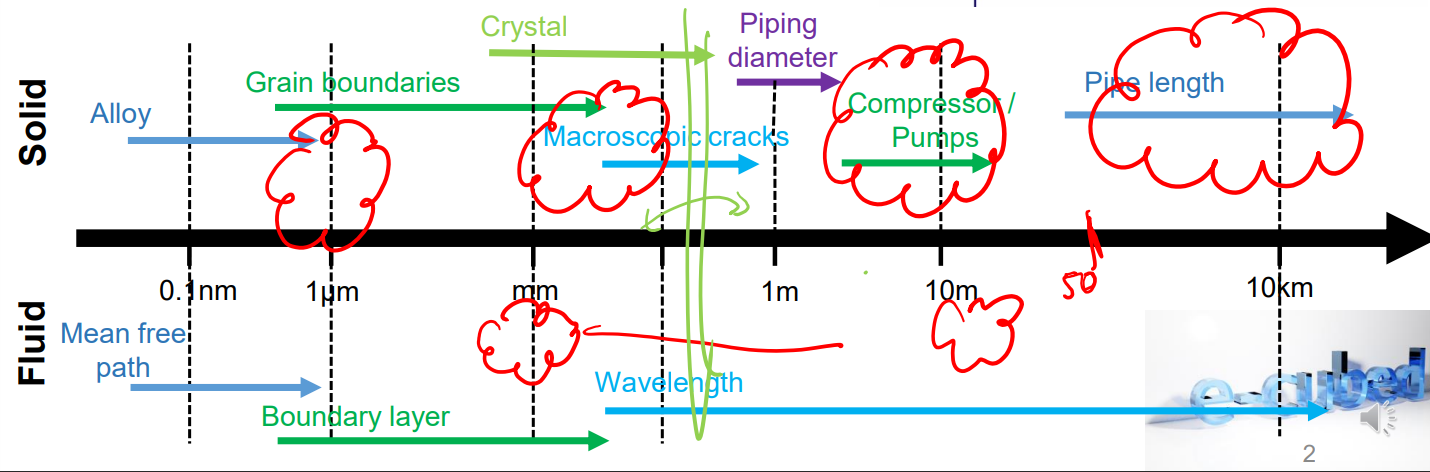
\includegraphics[width = \textwidth]{./img/figure1.png}
	\caption{Pressure pulsation in a piping system}
\end{figure}
\subsubsection{Cascade of length scales}
\begin{table}
	\begin{adjustbox}{width=\columnwidth,center}
		\begin{tabular}{@{}lll@{}}
			\toprule
			\textbf{Molecular}              & \textbf{Continuum}                            & \textbf{Structural}                     \\
			\midrule
			Material is made on this level  & Cracks operate on this level                  & Structures considered at this level     \\
			$< \SI{10}{\micro\meter}$       & $\SI{10}{\micro\meter} < x < \SI{10}{\meter}$ & $> \SI{10}{\meter}$                     \\
			Short range interactions        & Long range interactions                       & Whole scale interactions                \\
			Failure / corrosion / chemistry & Tune model - variables change                 & Long distance interaction               \\
			                                & continuously / smoothly (can account          & - vibration (waves transporting energy) \\
			                                & for discontinuous behaviour, e.g. crack)      &                                         \\
			\bottomrule
		\end{tabular}
	\end{adjustbox}
	\caption{Cascade of length scales}
\end{table}
\subsection{Complexity of the problem at different length scales}
Complexity of representation changes with the scale.
\begin{figure}[H]
	\centering
	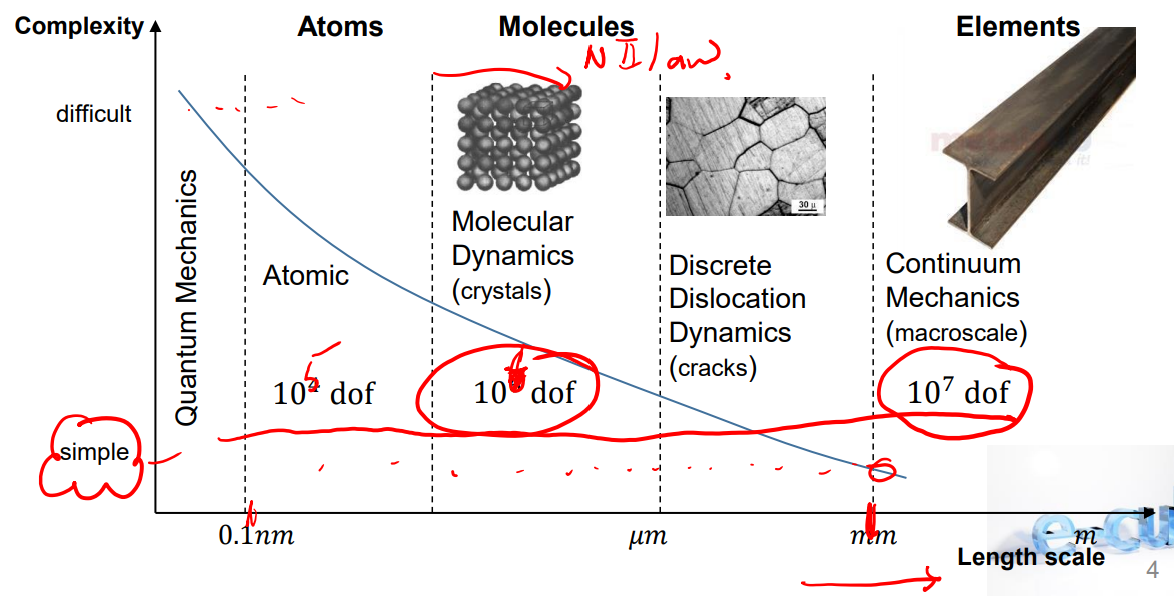
\includegraphics[width = \textwidth]{./img/figure2.png}
	\caption{Graph to show complexity against scale.}
\end{figure}
\subsection{Why focus on small scales?}
\begin{itemize}
	\item Small scale defects lead to crack initiation and propagation under external loading
	\item Failure can be corrected by changing material properties, for example, toughness
	\item Source of defects: complex chemical process (chemistry / corrosion) leads to corrosion at the surface
	\item Macroscale process is linked to microscale action
	\item Hypersonic flow - ionisation is non-continuum effect
	\item Analogy between defective liquids / solids
\end{itemize}
Note: turbulence is controlled by small vortices.
\subsubsection{Micrograph}
\begin{table}
	\centering
	\begin{tabular}{@{}ll@{}}
		\toprule
		\textbf{Domain}   & \textbf{Process}           \\
		\midrule
		Bulk              & Plasticity                 \\
		Internal boundary & Hydrogen embrittlement -   \\
		                  & plastic deformation / slip \\
		External boundary & Corrosion - chemistry      \\
		\bottomrule
	\end{tabular}
	\caption{Micrograph}
\end{table}
\begin{figure}[H]
	\centering
	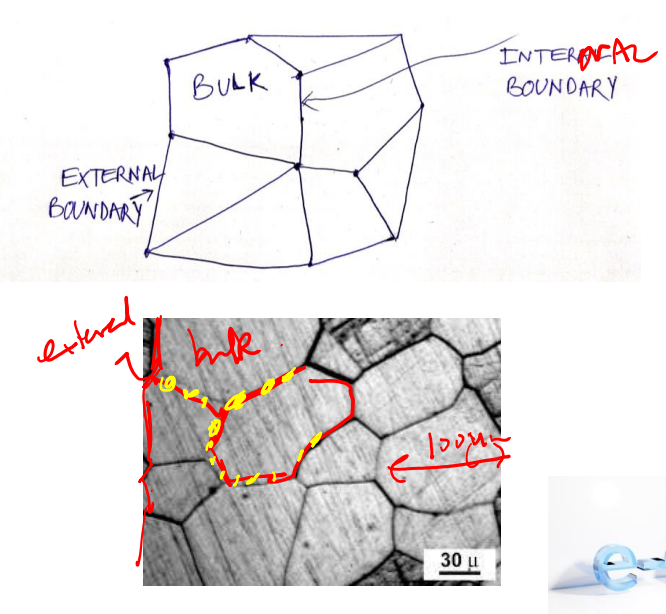
\includegraphics[width = 0.5\textwidth]{./img/figure3.png}
	\caption{Graph to show complexity against scale.}
\end{figure}
\subsubsection{Internal grain processes}
\begin{figure}[H]
	\centering
	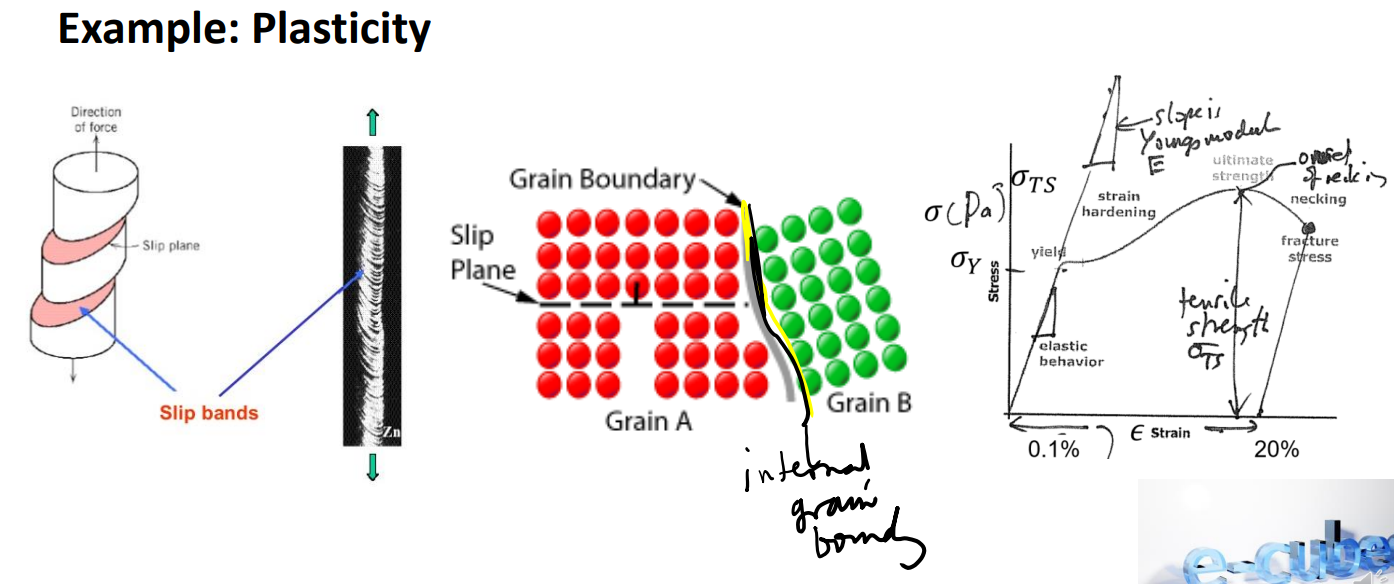
\includegraphics[width = 0.5\textwidth]{./img/figure4.png}
	\caption{Example of plasticity from internal grain process level.}
\end{figure}
\subsubsection{Internal boundary (hydrogen embrittlement - plastic deformation / slip)}
\begin{figure}[H]
	\centering
	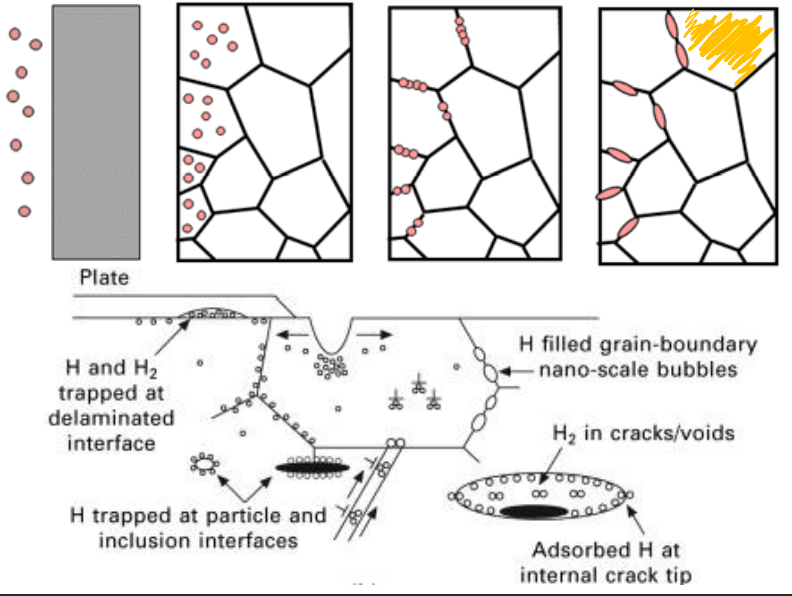
\includegraphics[width = 0.5\textwidth]{./img/figure5.png}
	\caption{Hydrogen embrittlement - plastic deformation / slip}
\end{figure}
\subsubsection{External boundary (corrosion)}
Corrosion happens over a long time and a range of scales. We need to understand how ions move around and interact with materials.
\begin{gather}
	\ce{Fe2 + (ag) + 2OH(ag) -> Fe(OH)_{2(s)}}\\
	\ce{4Fe(OH)_{2(s)} + O_{2(g)} + 2H2O_{(l)} -> Fe(OH)_{3(s)}}
\end{gather}
\begin{figure}[H]
	\centering
	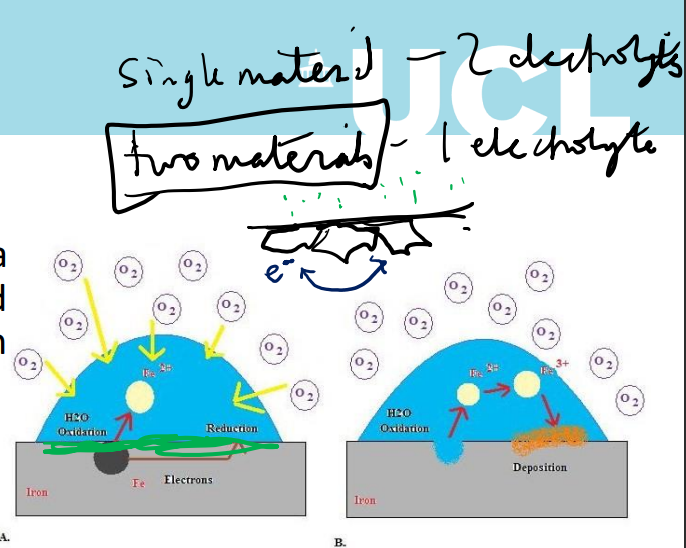
\includegraphics[width = 0.5\textwidth]{./img/figure6.png}
	\caption{Rust corrosion from grain boundary level.}
\end{figure}
\section{Categorisation of matter}
\begin{table}
	\centering
	\begin{tabular}{@{}lll@{}}
		\toprule
		\textbf{Matter} & \textbf{Modelling approach} &           \\
		\midrule
		Solid           & Atomistic                   & Continuum \\
		Gas             & Kinetic theory              & Continuum \\
		Liquid          & Molecular                   & Continuum \\
		\bottomrule
	\end{tabular}
	\caption{Categorisation of matter}
\end{table}
Switch between states are due to $p$, $V$ and $T$ and is represented by phase diagram. States of matter have been part of most religious and scientific texts for the last two thousand years, with water (aqua), fire (ignis), air (aer) and earth (terra) with the fifth being the void.
\section{Atomistic view of matter}
Typical length scale:
\begin{itemize}
	\item Diameter of atom is \SI{0.1}{\nano\meter} = \SI{1e-10}{\meter} = \SI{1}{angstrom}
	\item Nucleus diameter is \SI{1e-15}{\meter} (hydrogen) to \SI{15e-15}{\meter} (uranium-238)
\end{itemize}
\subsection{Bulk characteristic of materials}
The aim is to understand the relationship between the macrostructure and the microstructure. Key measures are:
\begin{itemize}
	\item Young's modulus $E = \left. \frac{\dif \sigma}{\dif \varepsilon} \right|_{\varepsilon \rightarrow 0}$
	\item Tensile stress: $\sigma_{TS}$
	\item Yields stress: $\sigma_{Y}$
	\item Ductility: $\epsilon_{T}$
\end{itemize}
It is important to understand the following:
\begin{table}
	\centering
	\begin{tabular}{@{}lll@{}}
		\toprule
		\textbf{Properties} &                                   & \textbf{Definition}                                \\
		\midrule
		Elastic modulus     & $E$ (\si{\pascal})                & Measure of material resistance to deformation.     \\
		Yield stress        & $\sigma_Y$ (\si{\pascal})         & Measure of stress at which the elastic behaviour   \\
		                    &                                   & disappears and plastic behaviour initiates.        \\
		Hardness            & HBW                               & Measure of material resistance to indentation      \\
		Creep               &                                   & Time-dependant deformation at high temperature     \\
		                    &                                   & and constant stress.                               \\
		Toughness           & $K$ (\si{\joule\per\meter\cubed}) & Resistance to crack propagation.                   \\
		Ductility           & $\epsilon_T$                      & Material's ability to undergo plastic deformation. \\
		\bottomrule
	\end{tabular}
	\caption{Key points on material properties}
\end{table}
How are they related to the microstructure?
\subsection{Newtonian model of matter}
Useful for biological, physical problems, solids, liquids and gases. This is based on a description of matter as a collection of point particles, an approach that is useful for gases, liquid and solids. The dynamics of the i-th molecule is:
\begin{gather}
	\underline{F}_i = \sum_{j,j} \neq \nabla U\left(x_i,x_j\right)
\end{gather}
Located at point $\underline{x}_i$ whose dynamics are:
\begin{gather}
	m_i \dfrac{\dif \underline{v}_i}{\dif t} = \underline{F}_i\\
	\underline{v}_i = \frac{\dif \underline{x}_i}{\dif t}
\end{gather}
The formulation requires the form of the interaction stated using the Lennard-Jones 6-12 potential:
\begin{gather}
	U = 4 \epsilon \left(\left(\frac{\sigma}{r}\right)^{12} - \left(\frac{\sigma}{r}\right)^6\right) + \dots
\end{gather}
The difficultly is that neighbourhood lists are kept and only sum over local interaction of molecules.
\begin{itemize}
	\item Not hard collision
	\item Time stepping fixed
	\item Potentials can be empirical or chosen to now slow down calculations
\end{itemize}
\begin{gather}
	U = U_{stretch} + U_{bend} + U_{torsion} + U_{vanderWaal} + U_{electro} + U_{cross}
\end{gather}
Research gaps:
\begin{itemize}
	\item Link between continuum and molecular
	\item Quantum - mechanical models
\end{itemize}
\subsection{Vibrational modes and energy}
Mechanical representation of matter. Molecules interact with their neighbours and fields. Interaction may be quite far, particularly when charges are important. We are familiar with how degrees of freedom influence properties of a gas, especially through the isentropic index. Energy is stored in various modes of vibration e.g. gas. This is called classical molecular dynamics.
\subsection{Molecular description of material properties}
\subsubsection{Primary bonds}
Ionic and covalent bonds are extremes with most (electron distribution) bonds lying between (polar covalent)
\begin{figure}[H]
	\centering
	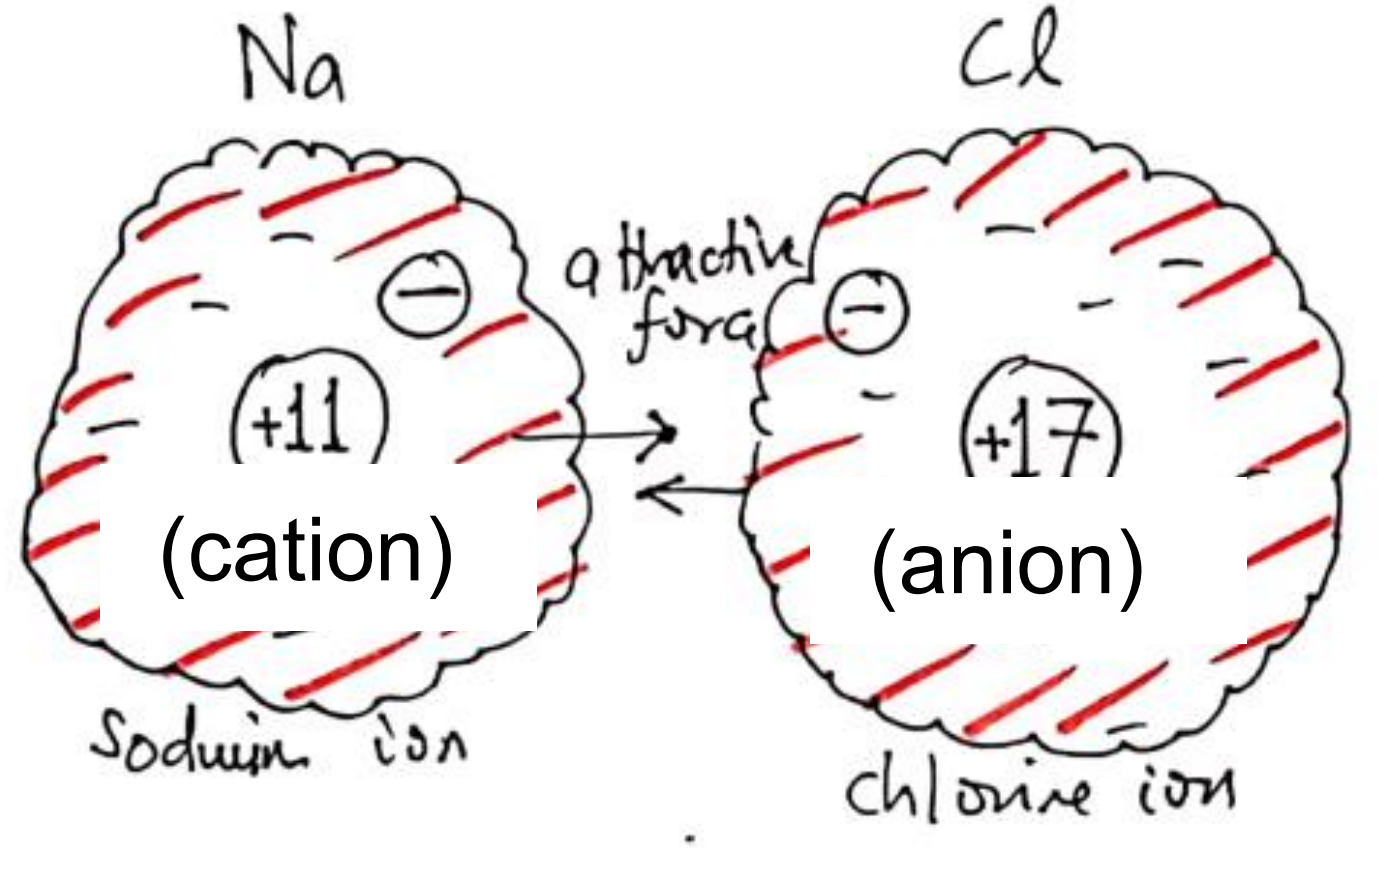
\includegraphics[width = 0.5\textwidth]{./img/figure7.png}
	\caption{Ionic bond (electrovalence)}
\end{figure}
\begin{gather}
	F = \frac{q_1 q_2}{4\pi \epsilon_0 r^2}\\
	U = U_i - \frac{q^2}{4\pi\epsilon_0 r} + \frac{B}{r^n}
\end{gather}
\begin{figure}[H]
	\centering
	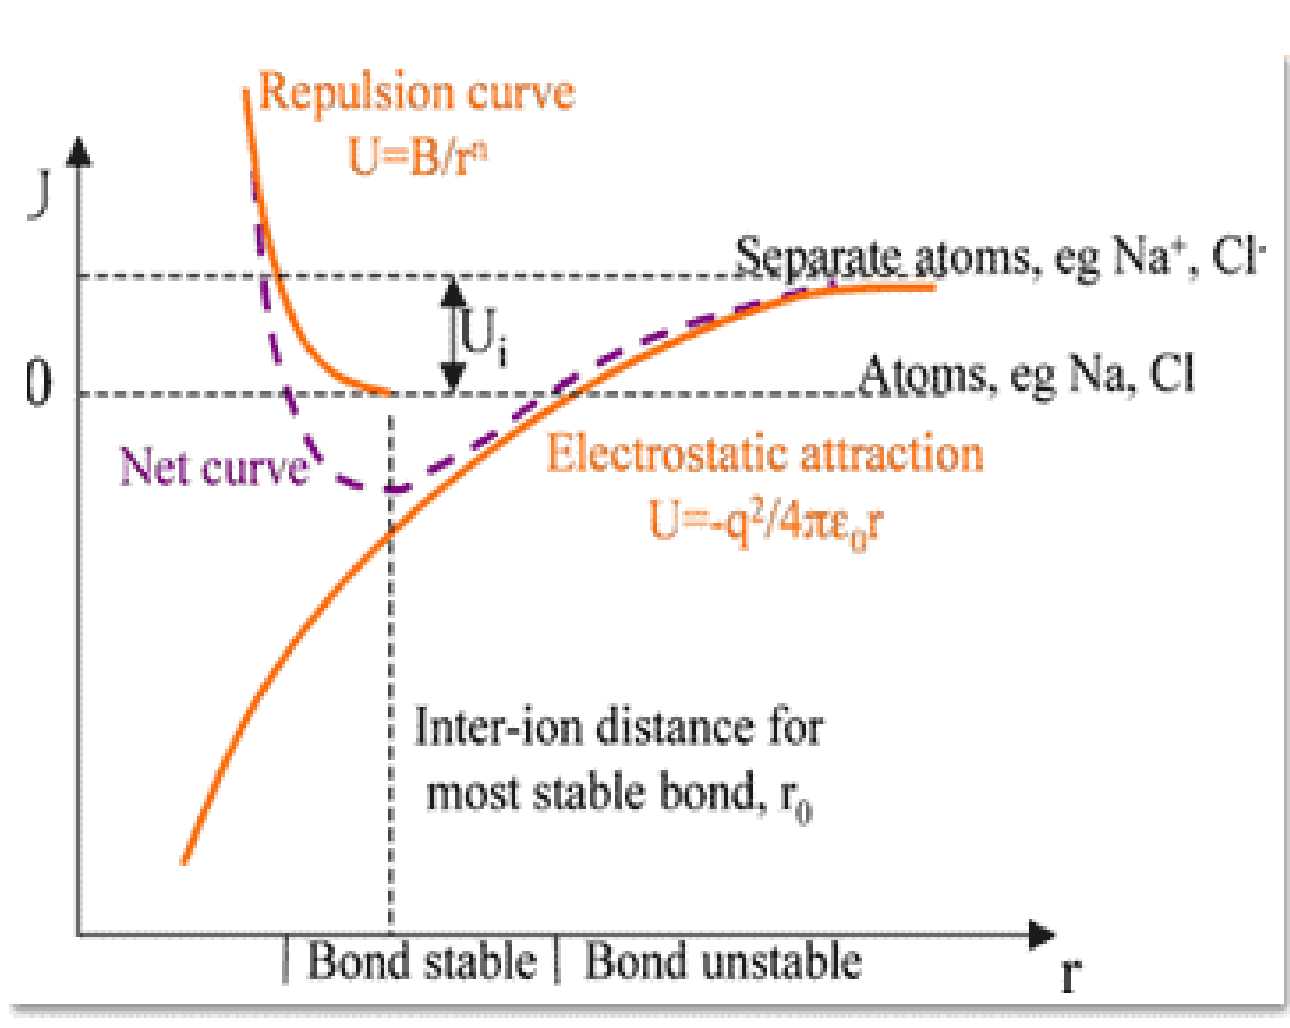
\includegraphics[width = 0.5\textwidth]{./img/figure8.png}
	\caption{Bond stability.}
\end{figure}
\begin{figure}[H]
	\centering
	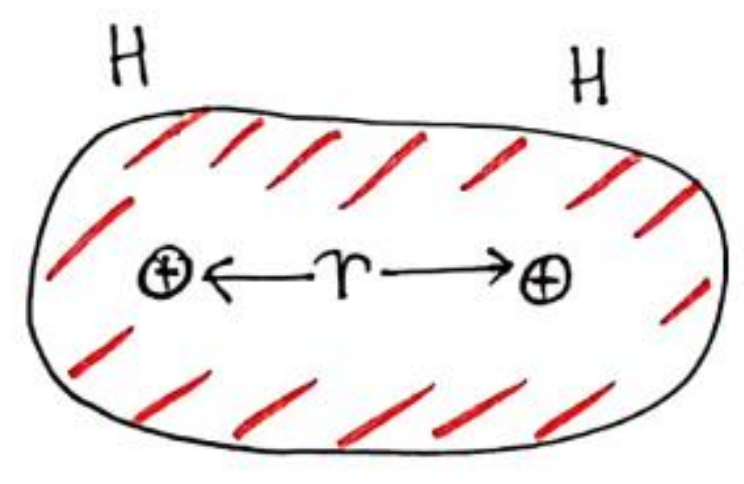
\includegraphics[width = 0.5\textwidth]{./img/figure9.png}
	\caption{Covalent bond (covalence). Note the overlap of electron orbit.}
\end{figure}
\begin{gather}
	U = -\frac{A}{r^m} + \frac{B}{r^n}, \, m<n
\end{gather}
\begin{figure}[H]
	\centering
	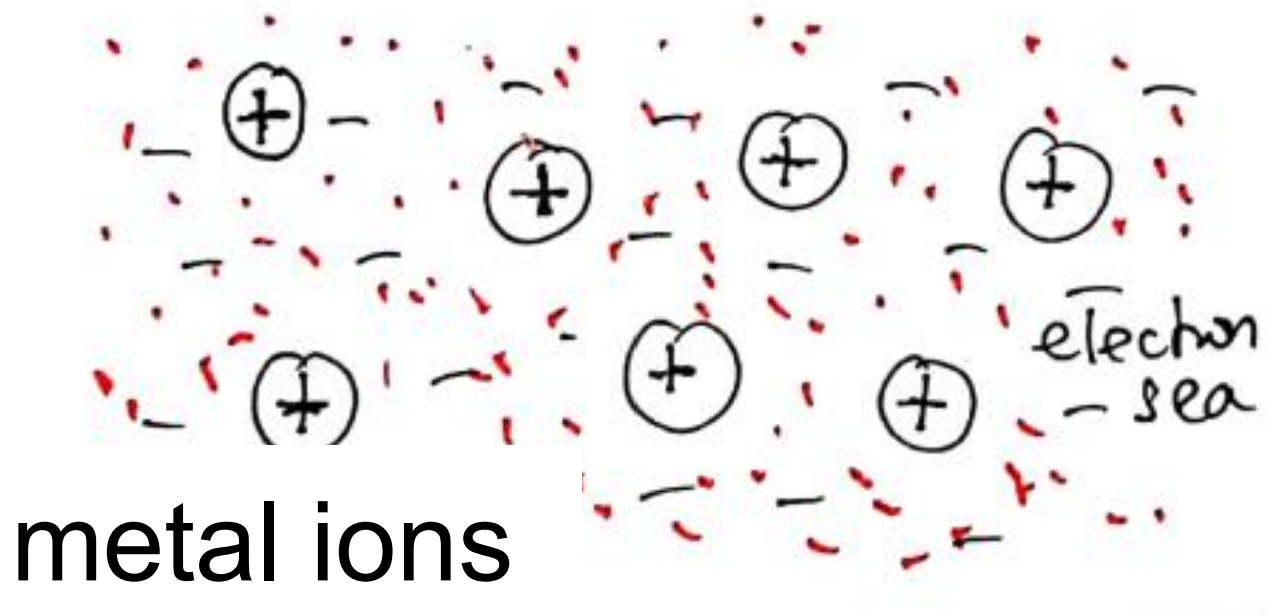
\includegraphics[width = 0.5\textwidth]{./img/figure10.png}
	\caption{Metallic bond (electron cloud).}
\end{figure}
\begin{gather}
	e = \SI{1.6e-19}{C}\\
	\epsilon_0 = \SI{8.8e-12}{Nm^2C^{-2}}\\
	\SI{1}{eV} = \SI{1.6e-19}{J}
\end{gather}
\subsubsection{Secondary bonds}
The secondary bonds are important - without them many gases would not condense. The relative displacement of the positive and negative charge gives rise to a dipolar force. This gives rise to an attractive force. Most usual form is the Lennard Jones 6-12 potential.
\begin{gather}
	U = -\frac{A}{r^6} + \frac{B}{r^n}
\end{gather}
\begin{figure}[H]
	\centering
	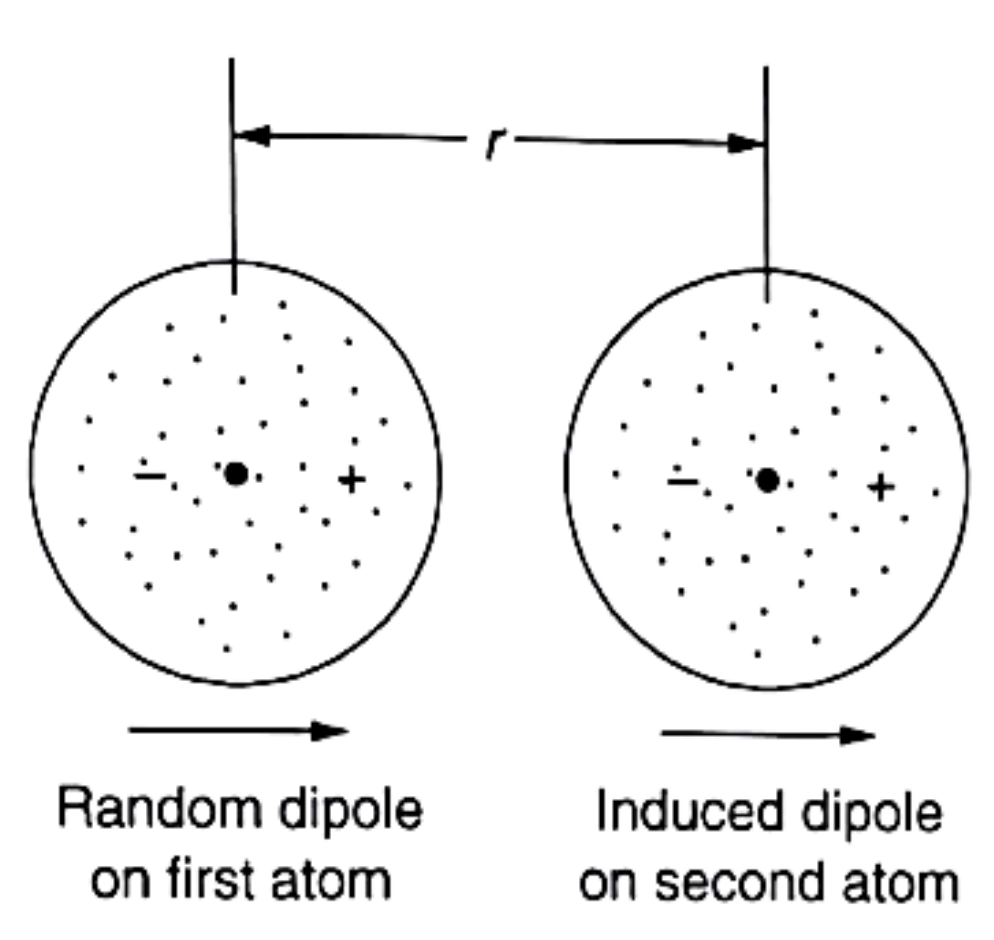
\includegraphics[width = 0.5\textwidth]{./img/figure11.png}
	\caption{Secondary bonds. Note: long range attractive force -  dipole-dipole interactions. Overlapping electron orbits - repulsive.}
\end{figure}
\subsubsection{Physical basis of Young's Modulus}
Classical mechanics:
\begin{gather}
	m\frac{\dif v}{\dif t} = \frac{\dif U }{\dif r}
\end{gather}
where $U$ is the potential energy. At equilibrium:
\begin{gather}
	\frac{\dif U}{\dif r } = 0
\end{gather}
so that close to this point, the energy potential can be expanded to give:
\begin{gather}
	m \frac{\dif^2 r }{\dif t^2} = \left(\frac{\dif^2 U}{\dif r^2}\right)\left(r-r_0\right)
\end{gather}
Around equilibrium point:
\begin{gather}
	F = S_0 \left(r - r_0\right)\\
	S_0 = -\frac{\dif^2 U}{\dif r^2}
\end{gather}
The stress is:
\begin{gather}
	\sigma = N S_0 \left(r - r_0\right) = \frac{S_0\left(r-r_0\right)}{r_0^2}
\end{gather}
The Young's modulus is:
\begin{gather}
	E = \frac{\sigma}{\epsilon} = \frac{S_0}{r_0}
\end{gather}
Estimate:
\begin{gather}
	S_0 = \frac{\alpha q^2}{4\pi\epsilon_0r^2}\\
	E = \frac{\sigma}{\epsilon} = - \frac{\frac{\dif^2 U}{\dif r^2}}{r_0} = \frac{\delta e^2}{4\pi\epsilon_0r_0^4}
\end{gather}
Atom spacing:
\begin{gather}
	\overline{r}_0 \approx 8.54
\end{gather}
\begin{figure}[H]
	\centering
	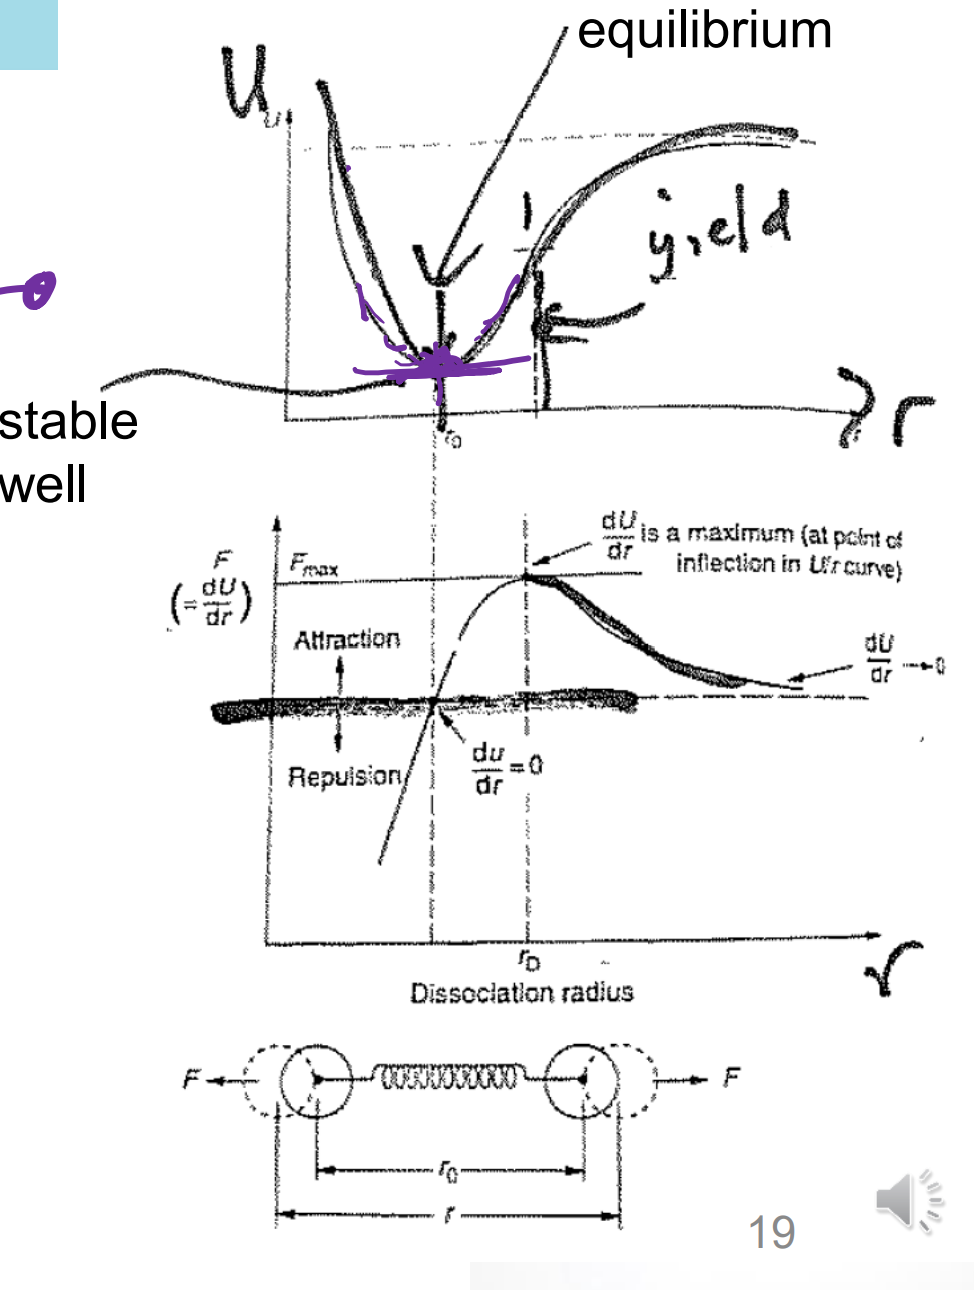
\includegraphics[width = 0.5\textwidth]{./img/figure12.png}
	\caption{Young's modulus from atomic perspective.}
\end{figure}
\subsubsection{Comparison between molecular and macroscopic measurements}
\begin{table}[H]
	\centering
	\begin{tabular}{@{}llll@{}}
		\toprule
		\textbf{Bond type} & $S_0$ / \si{Nm^{-1}} & \textbf{Young's modulus estimate} & \textbf{Measurement}       \\
		                   &                      & $E$ / \si{\giga\pascal}           &                            \\
		\midrule
		Covalent           & 50 - 180             & 200 - 1000                        & 1000 (diamond)             \\
		Metallic           & 15 - 75              & 60 - 300                          & 200 (nickel)               \\
		Ionic              & 8 - 24               & 32 - 96                           & 15 - 91 (alkali halides)   \\
		H-Bond             & 2 - 3                & 8 - 12                            & 9.1 (ice)                  \\
		van der Waals      & 0.5 - 1              & 2 - 4                             & 0.01 - 2 (rubber to nylon)
	\end{tabular}
	\caption{Comparison between molecular and macroscopic measurements.}
\end{table}
\subsubsection{Estimation of yield stress}
Returning to the molecular model since:
\begin{gather}
	U = \epsilon \left(-\frac{A}{r^6} + \frac{B}{r^{12}}\right)\\
	U'' = \epsilon \left(- \frac{6\times 7A}{r^8} + \frac{12\times 13B}{r^{14}}\right)
\end{gather}
Then, maximum stress is:
\begin{gather}
	\sigma_Y \approx \frac{E}{8}
\end{gather}
Therefore:
\begin{gather}
	\frac{\sigma_Y}{E} ~ \frac{1}{8}
\end{gather}
This estimated ratio is good for ceramics, but not good for metals. So what is missing from a molecular description?
\begin{figure}[H]
	\centering
	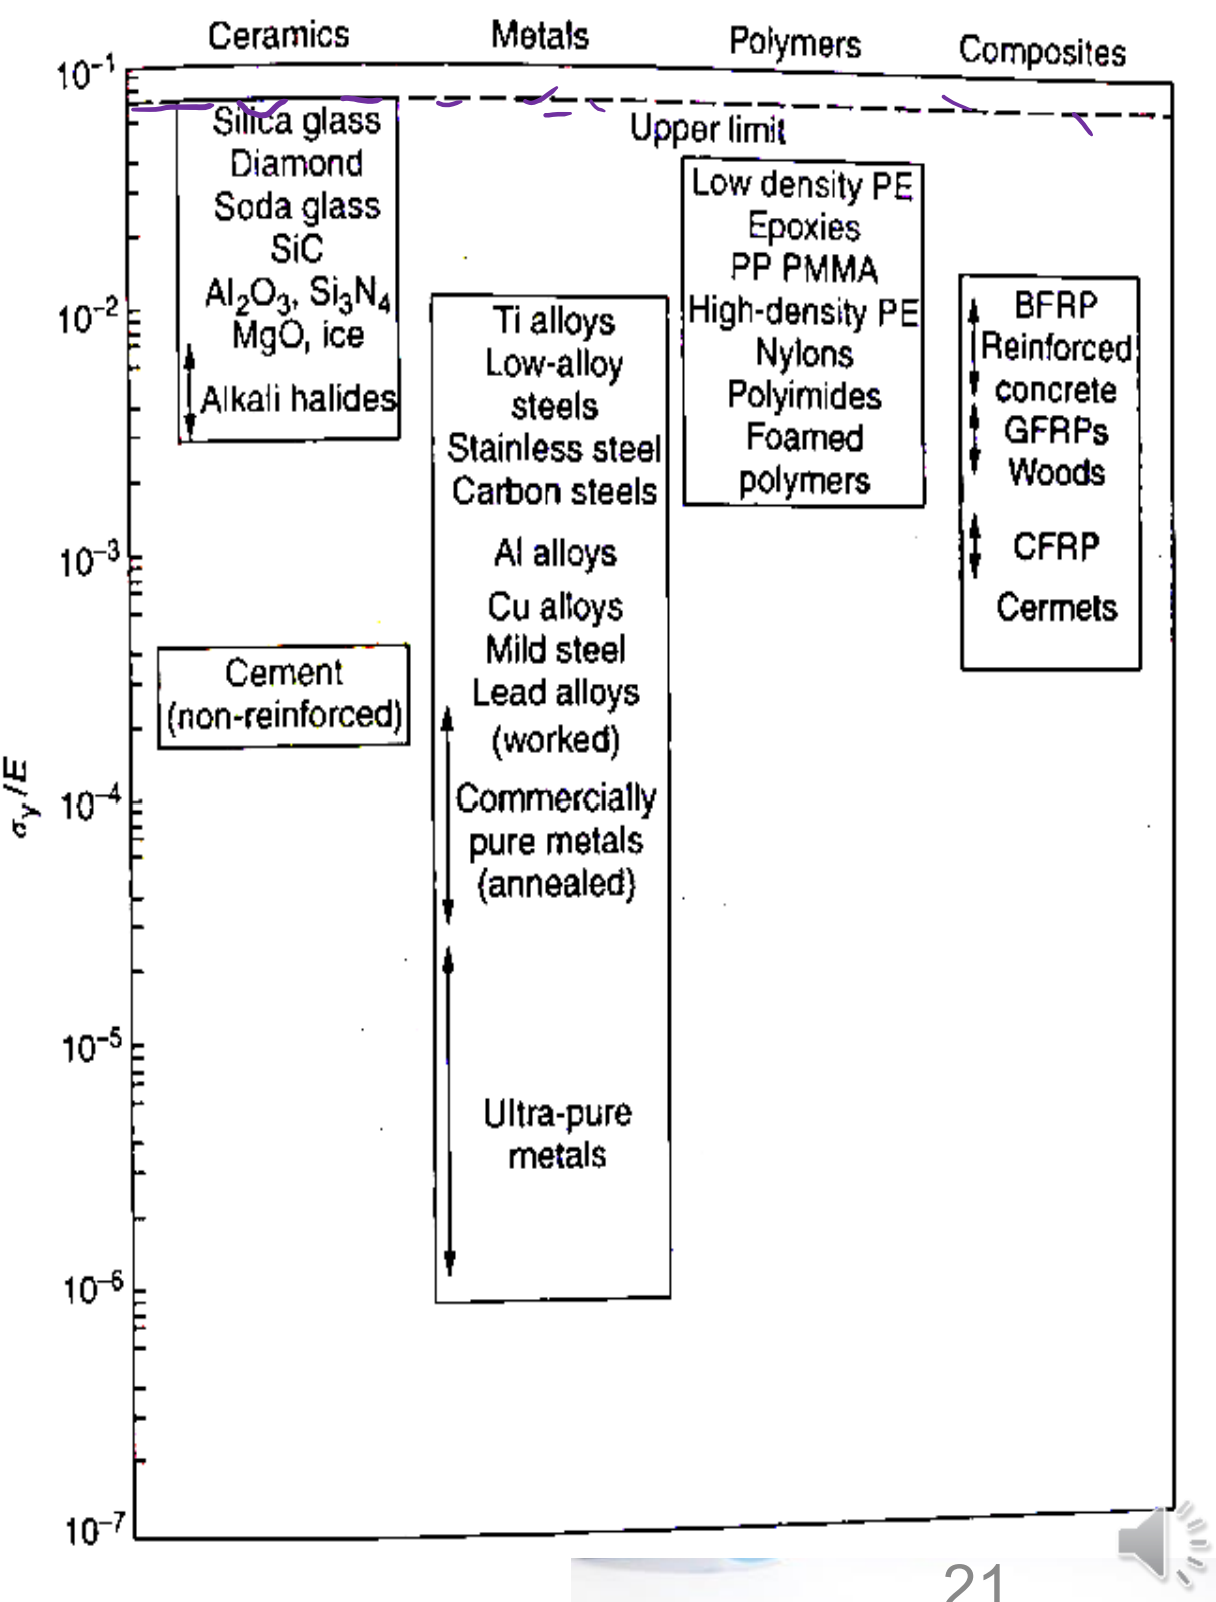
\includegraphics[width = 0.5\textwidth]{./img/figure13.png}
	\caption{Graph to show yield stress ratio for different materials.}
\end{figure}
\subsection{Material classification}
\begin{itemize}
	\item Metals
	      \begin{itemize}
		      \item Ferrous metals and alloys
		      \item Non ferrous metals and alloys
		      \item (focus on here)
	      \end{itemize}
	\item Polymeric (non metallic, non crystalline)
	      \begin{itemize}
		      \item Thermoplastic plastics
		      \item Thermoset plastics
		      \item Elastomers
	      \end{itemize}
	\item Ceramics
	      \begin{itemize}
		      \item Glass
		      \item Diamond
		      \item Glass ceramics
	      \end{itemize}
	\item Composites (everything else)
	      \begin{itemize}
		      \item Metal-matrix composites
		      \item Sandwich structures
		      \item Concrete
	      \end{itemize}
\end{itemize}
\subsubsection{Three common configurations}
\begin{table}[H]
	\centering
	\begin{tabular}{@{}llll@{}}
		\toprule
		\textbf{Type} & \textbf{Name}               & \textbf{Description}      & \textbf{Example}             \\
		\midrule
		BCC           & Body centred cube - 2 atoms & Harder and less malleable & Lithium, Sodium, Potassium   \\
		              &                             & Packing factor 0.68       & Chromium, Barium, Alpha-iron \\
		FCC           & Face centred cube           & malleable, softer 0.74    & Copper, Gold, Aluminium      \\
		              &                             &                           & Iridium, Lead, Nickel, etc.  \\
		HCP           & Hexagonal close packed      & 6 atoms                   & Cadmium, Magnesium, Titanium \\
		              &                             & Packing ratio 0.74        & Zinc, Zirconium              \\
		\bottomrule
	\end{tabular}
	\caption{Configurations of atoms.}
\end{table}
\subsubsection{Solidification and crystal growth}
Under normal circumstances, crystal growth starts at many nucleation points. Solidification leads to crystals growing and stop growing when they meet another crystal. A crystal is usually called a grain. The boundary between grains is the grain boundary where structure is disordered. This is controlled using nucleation points and directional solidification and liquid freezing-dendritic growth and shrinkage occurs during cooling.
\begin{figure}[H]
	\centering
	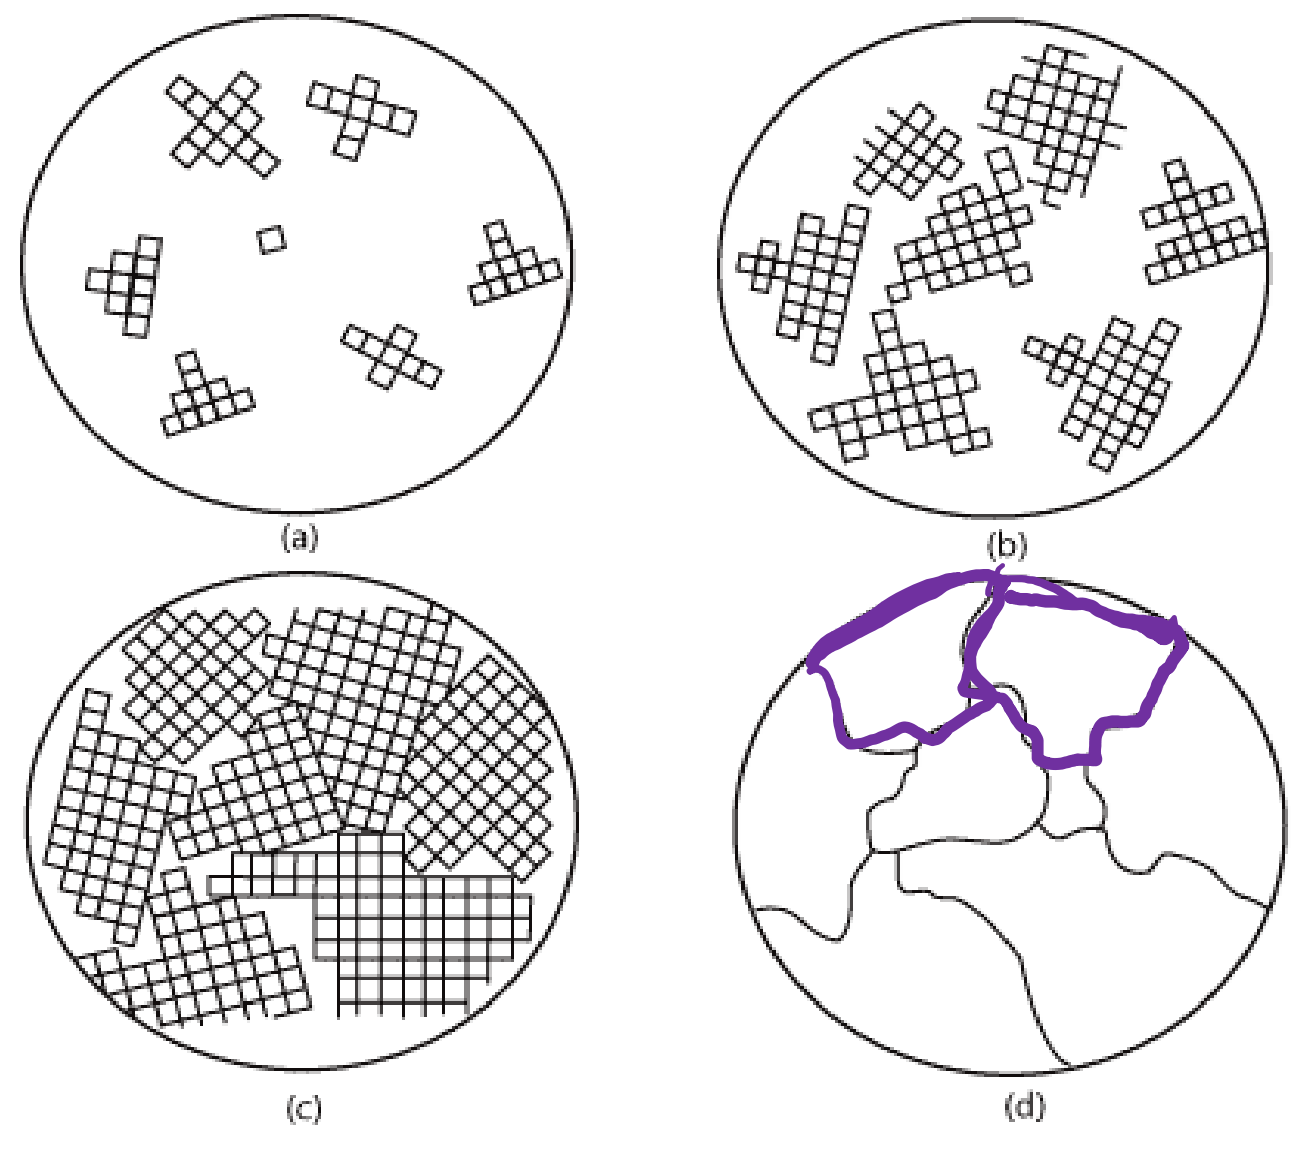
\includegraphics[width = 0.6\textwidth]{./img/figure14.png}
	\caption{Nucleation of crystals.}
\end{figure}
\subsubsection{Crystal defects}
Three types of defects:
\begin{enumerate}
	\item Point defects: which are places where an atom is missing or irregularly placed in the lattice structure. Point defects include lattice vacancies, self interstitial atoms, substitution impurity atoms and interstitial impurity atoms
	\item Linear defects: which are groups of atoms in irregular positions. Linear defects are commonly called dislocations
	\item Planar defects: which are interfaces between homogeneous regions of the material. Planar defects include grain boundaries, stacking faults and external surfaces
\end{enumerate}
\subsubsection{Atomistic view of plastic deformation}
Elastic deformation - stress is small, the metal can recover to initial state when the stress is removed. This involves stretching the bonds but atoms do not mover over one another.

Plastic deformation - stress is large, plastic deformation involves the breaking of a limited number of atomic bonds by the movement of dislocations. Since the energy required to move is lowest along the densest planes of atoms, dislocations have a preferred direction of travel within a grain of the material. This results in slip that occurs along parallel planes within the grain. These parallel slip planes group together to form slip bands. A slip band appears as a single line under the microscope, but it is in fact made up of closely spaced parallel slip planes as shown in the image.
\begin{figure}[H]
	\centering
	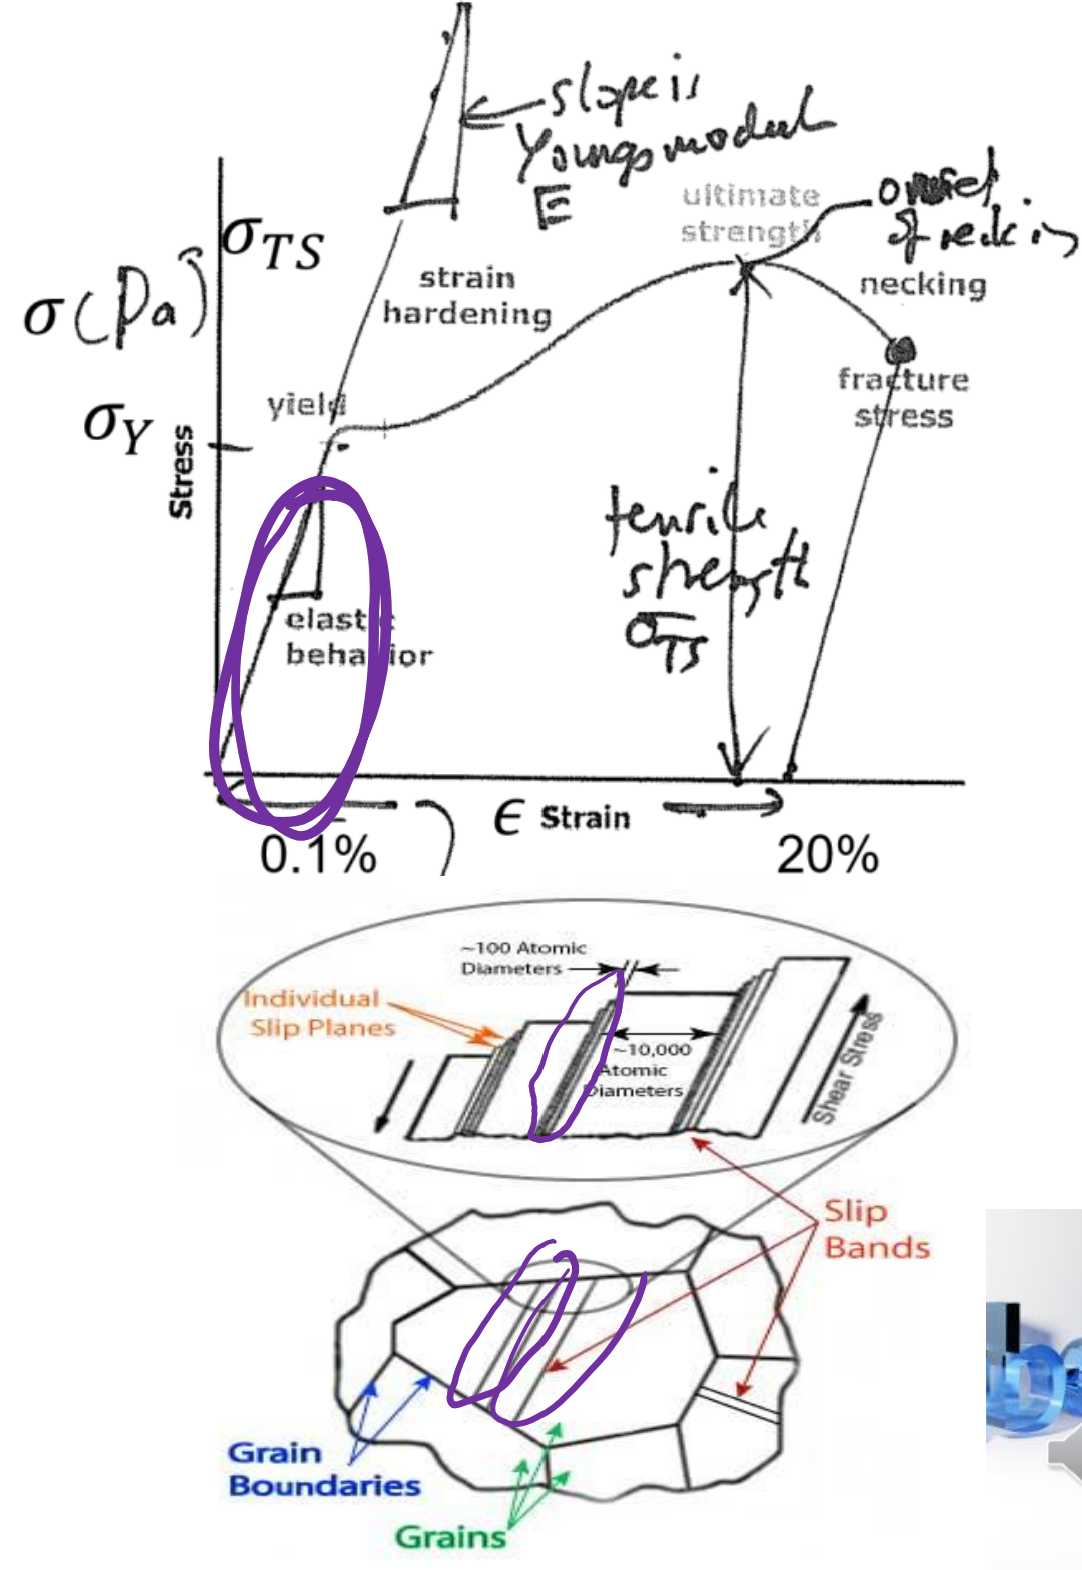
\includegraphics[width = 0.5\textwidth]{./img/figure15.png}
	\caption{Stress-strain curve.}
\end{figure}
\subsubsection{Fatigue crack initiation}
The life of a fatigue crack has two parts, initiation and propagation. Dislocations play a major role in the fatigue crack initiation phase. It has been observed in laboratory testing that after a large number of loading cycles dislocation pule up and form structures called persistent slip bands. Initiation has a molecular origin.
\subsubsection{Topological change in crystal structure}
\begin{figure}[H]
	\centering
	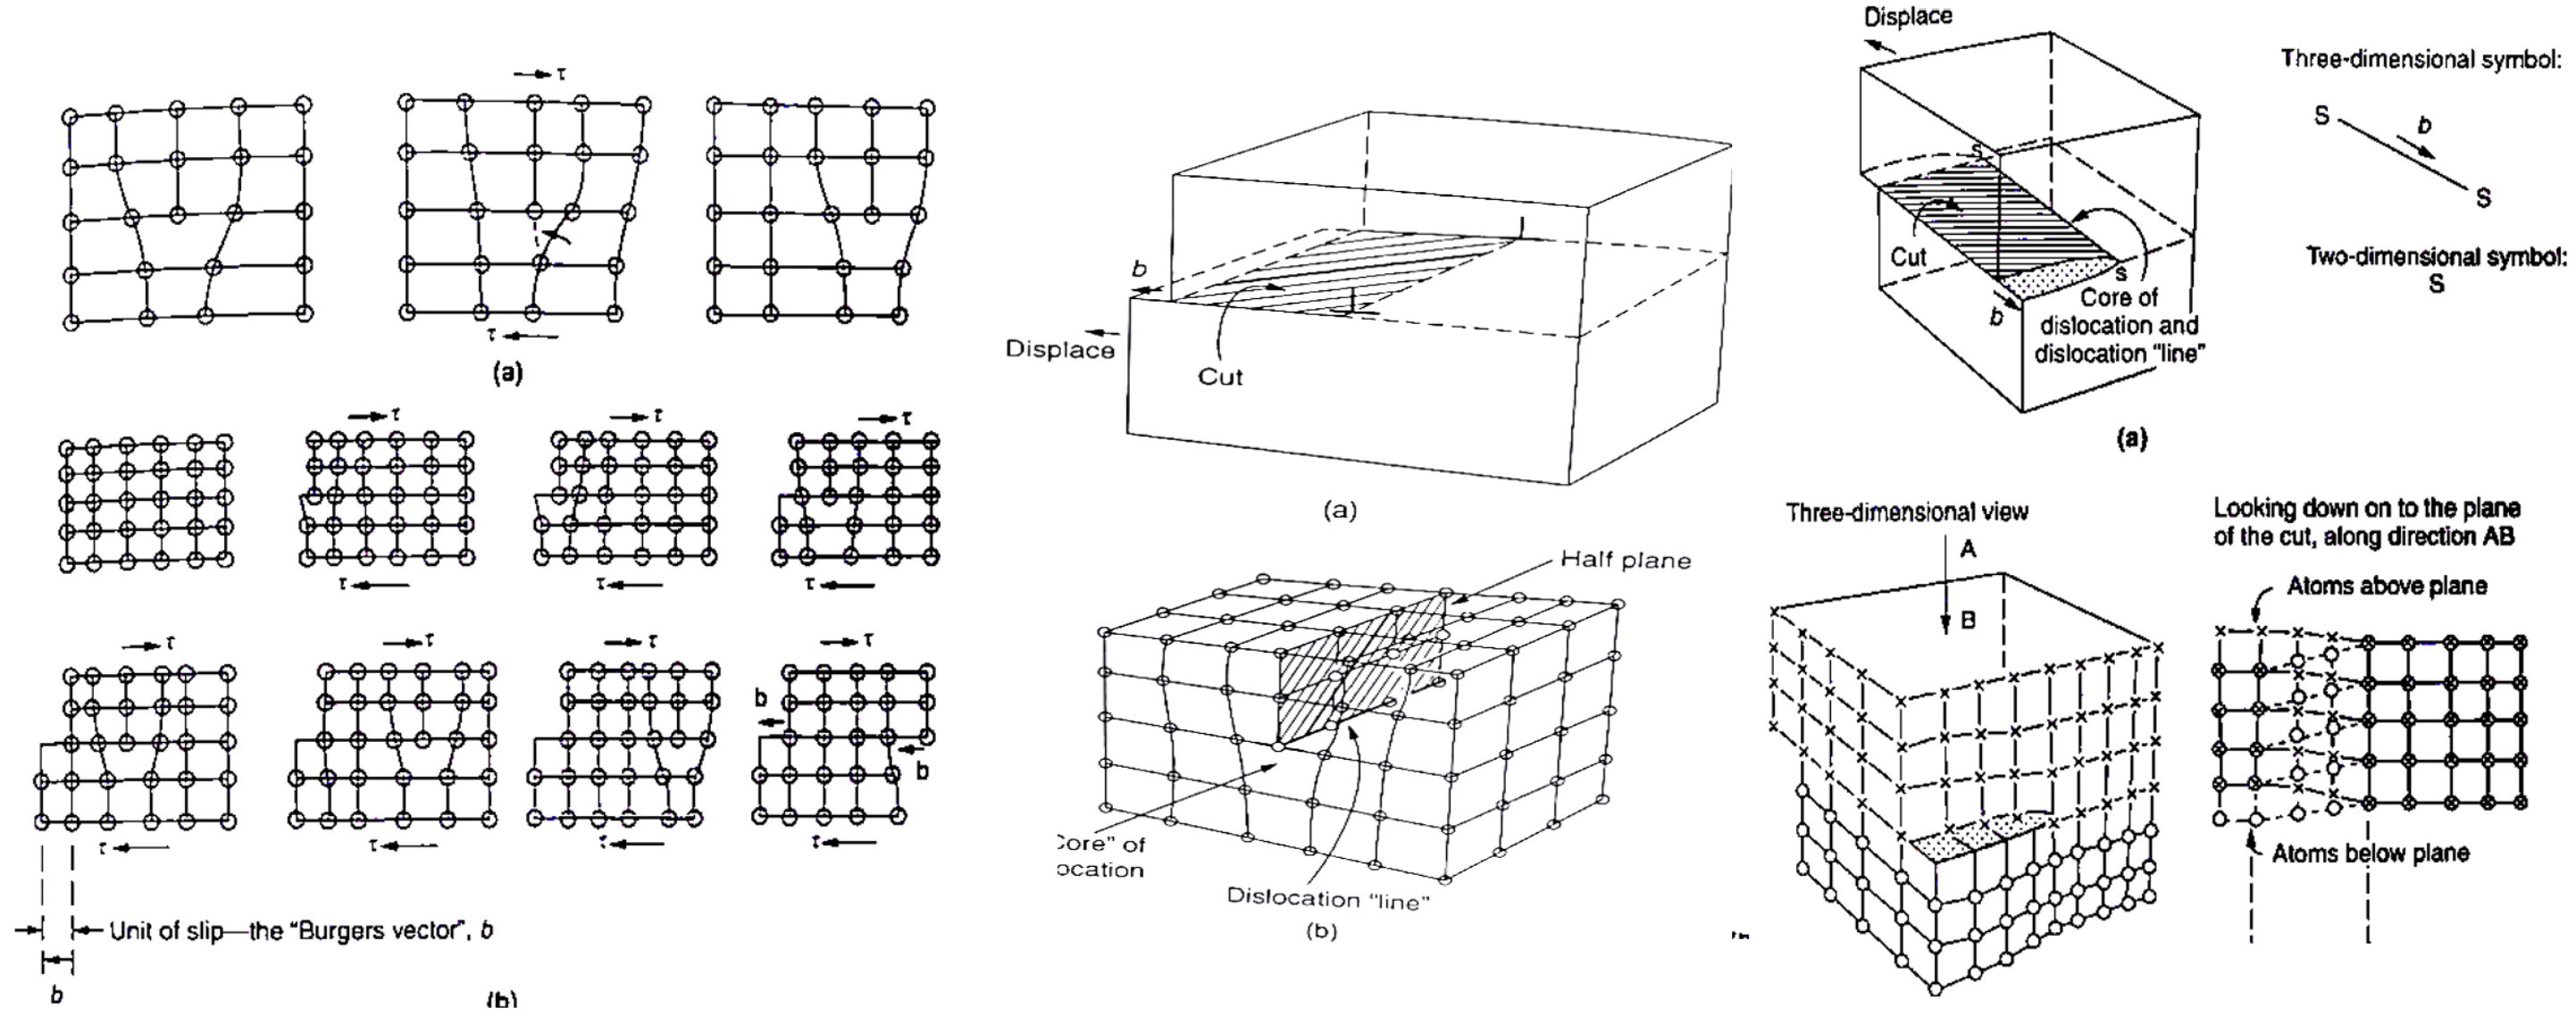
\includegraphics[width = 0.5\textwidth]{./img/figure16.png}
	\caption{Topological changes in crystal structure.}
\end{figure}
\section{Kinetic theory of gases}
Statistical 19th century view of macroscopic properties of gas. Boltzmann and colleagues developed new techniques to describe matter. Heavily influenced the theory of turbulence $\leftarrow$ based on kinetic theory of a gas.

$p = \rho RT$ origin with statistical theory.

This is an excellent macroscopic model of matter. The problem is that it does not work well for low pressure, high pressure or when density is low (and continuum concepts don't work).
\subsection{Speed of molecules}
Results tell us about average speed but not the distribution.
\begin{gather}
	n_v\left(E\right) = n_0 e^{-\frac{E}{k_B T}}
\end{gather}
where, $n_v\left(E\right)$ is the Boltzmann distribution which coups a lot. The speed of the molecules satisfies the Maxwell-Boltzmann distribution.
\begin{gather}
	f\left(v\right) = 4\pi \left(\frac{m}{2\pi k_B T}\right)^3 v^2 \exp{\left(-\frac{mv^2}{2k_B T}\right)}
\end{gather}
\begin{figure}[H]
	\centering
	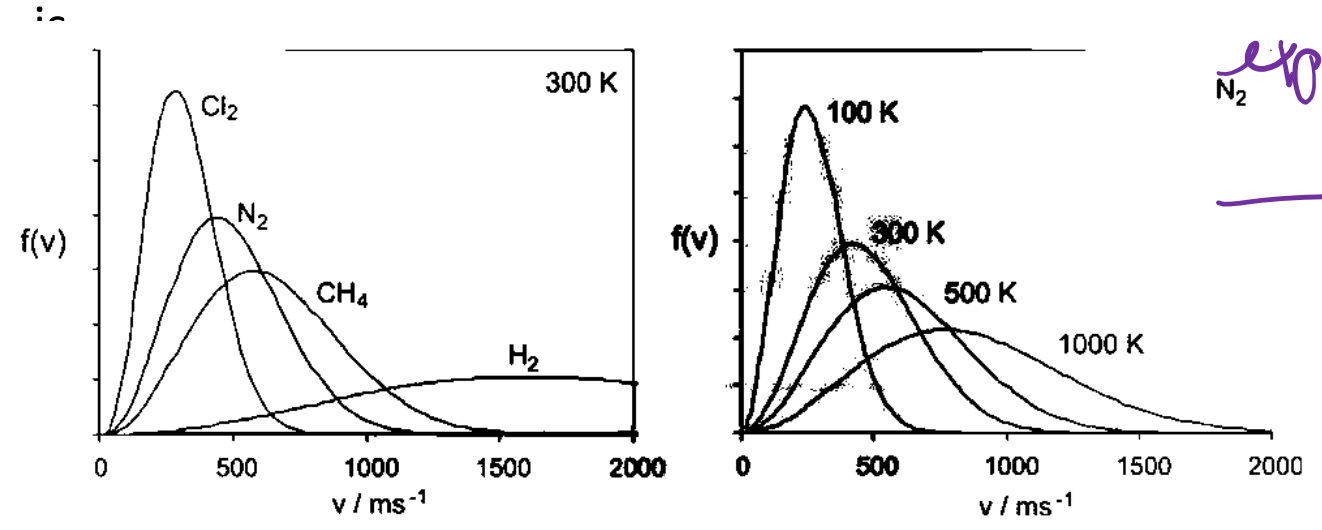
\includegraphics[width = 0.7\textwidth]{./img/figure17.png}
	\caption{Speed of molecules.}
\end{figure}
\subsection{Equations of state of real gases}
The molecular continuum view of matter are linked. Virial equation:
\begin{gather}
	pV = nRT\left(1 + \frac{B}{V_m} + \frac{C}{V_m^2} + \dots\right)
\end{gather}
where $B$, $C$ are the second and third virial coefficients. Van der Waals equation:
\begin{gather}
	\left(p + a\frac{n^2}{V^2}\right)\left(V - nb\right) = nRT \textrm{ or}\\
	P = \frac{nRT}{V- nb} - a \frac{n^2}{V^2}
\end{gather}
$n$ is the number of moles. $nb$ is the volume excluded since molecules cannot overlap. $\frac{an^2}{V^2}$ pressured reduced due to attractions between pairs of molecules.
\subsubsection{Critical constants for van der Waals equation}
Solving these two equations in two unknowns (temperature and molar volume) gives the critical temperature and critical molar volume:
\begin{gather}
	T_c = \frac{8a}{27Rb}\\
	V_c = 3b
\end{gather}
\subsubsection{Van der Waals}
\begin{figure}[H]
	\centering
	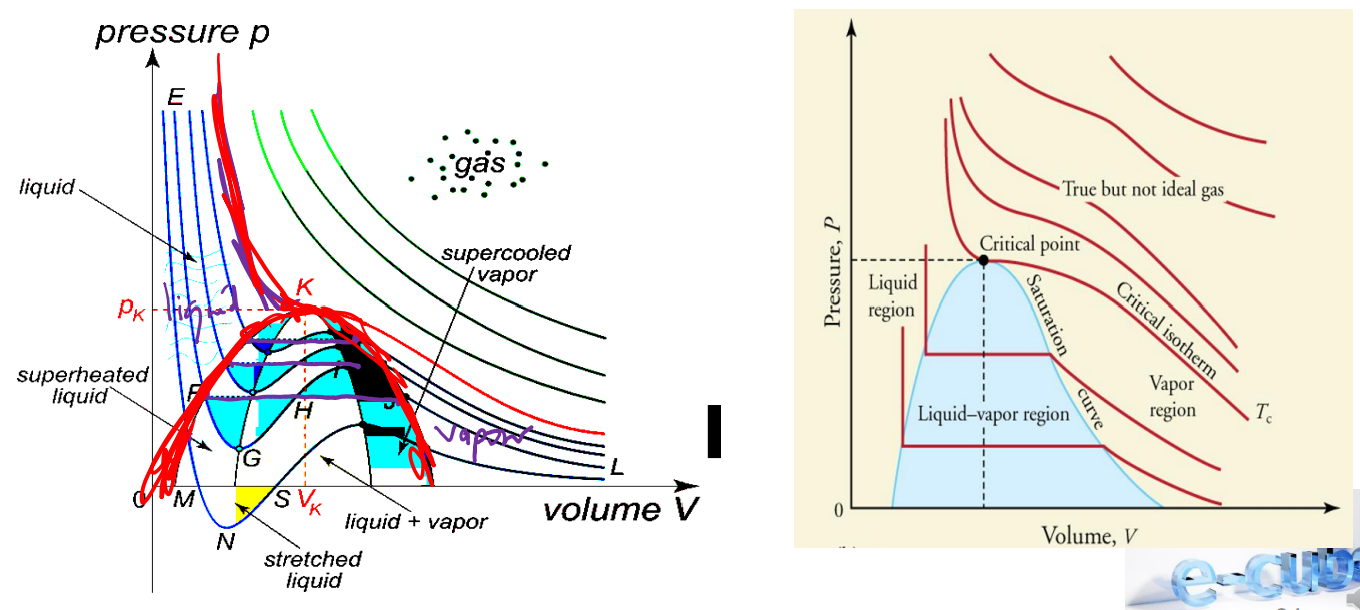
\includegraphics[width = 0.7\textwidth]{./img/figure18.png}
	\caption{Van der Waals.}
\end{figure}
\subsubsection{Link between molecular and microscopic}
Most of the important 19th century breakthroughs were determining link between macroscopic (could be seen) and microscopic (could not be seen). For example, Brownian motion:
\begin{gather}
	\frac{RT}{5\pi\mu dN_A} = D = \lim_{t\rightarrow \infty} \frac{\left(x^2\right)}{2t} \approx \SI{10e-10}{\meter\squared\per\second}
\end{gather}
This represented a link between Avogadro's constant and macroscopic movement of particles. Here $N_A = \SI{6e23}{\per\mole}$. Theory by Einstein (1905) and Sutherland (1905). Millikans experiments: determination of the charge on an electron. The link between molecular and microscopic last areas of modern science to be worked out.
\subsubsection{Einstein theory and Millikans experiment}
Based around kinetic theory of gases and momentum change due to collision. Pressure is a manifestation of a:
\begin{gather}
	P = \frac{2}{3}\frac{N}{V}\frac{1}{2}m_0 \overline{v}^2\\
	\therefore PV = nRT = \frac{N}{N_a}RT = Nk_BT\\
	\therefore KE = \frac{3}{2}Nk_bT = \frac{3}{2}nRT = \frac{NDF}{2}nRT
\end{gather}
where $NDF$ is number of degrees of freedom.
\subsubsection{Model assumptions}
\begin{itemize}
	\item No intermolecular forces between the gas particles
	\item The volume occupied by the particles is negligible compared to the volume of the container they occupy
	\item The only interactions between the particles and with the container walls are perfectly elastic collisions.
	\item Real gas, the atoms or molecules have a finite size, and at close range they interact with each other through a variety of intermolecular forces, including dipole-dipole interactions, dipole induced dipole interactions and van der Waal's (induced dipole - induced dipole) interactions
	\item When applied to real gases, the ideal gas model breaks down when molecular size effects or intermolecular forces become important. This occurs under conditions of high pressure , when the molecules are forced close together and therefore interact strongly, and at low temperatures, when the molecules are moving slowly and intermolecular forces have a long time to act during a collision
\end{itemize}
The pressure at which the ideal gas model starts to break down will depend on the nature and strength of the intermolecular forces between the gas particles, and therefore on their identity. The ideal gas model becomes more and more exact as the pressure is lowered, since at very low pressures the gas particles are widely spaced apart and interact very little with each other.
\begin{gather}
	\textrm{number density } = \frac{N}{V} = \frac{nN_A}{V}\\
	\Delta p_x = \left(2mv_x\right)\left(\frac{1}{2}\frac{nN_a}{V}Av_x \Delta t\right) = \frac{nMAv_x^2 \Delta t}{V}\\
	p = \frac{F_x}{A} = \frac{nMv_x^2}{V}
\end{gather}
\section{Chemistry for engineers}
Chemistry has a molecular origin. The engineering challenge is how to include chemistry into multi-physics problems. Chemistry might be simple:
\begin{gather}
	\ce{NaOH + HCl -> NaCl + H2O}
\end{gather}
\part{Extreme Temperature}
\chapter{How to cool very hot surfaces}
\section{Introduction}
\begin{table}[H]
    \centering
    \begin{tabular}{@{}lll@{}}
        \toprule
        \textbf{Context} & \textbf{Material development} & \textbf{Design}\\
        \midrule
        Gas turbine engines & Material development & TBC\\
        & manufacturing techniques & air cooling\\
        Re-entry spacecraft & Surface properties & Angle of attack\\
        & ablation & changing geometry\\
        Silicon processors & None really - still with silicon & Clamp on cooling system\\
        & with an adhesive metal plate\\
        \bottomrule
    \end{tabular}
    \caption{Introduction.}
\end{table}
\section{Jet engines}
Purpose is to convert chemical energy into linear momentum (IC engine - chemical energy into pressure).
\begin{figure}[H]
    \centering
    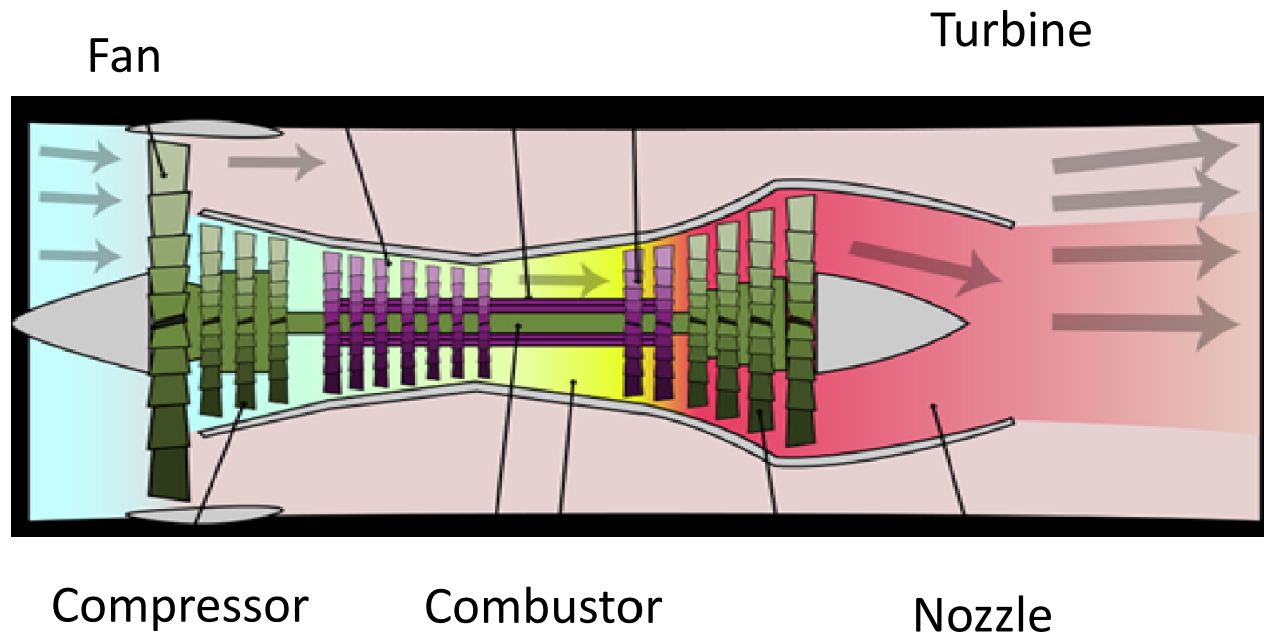
\includegraphics[width = 0.8\textwidth]{img/figure19.png}
    \caption{Jet engine.}
\end{figure}
\subsection{Brayton (or Joule) cycle}
\begin{figure}[H]
    \centering
    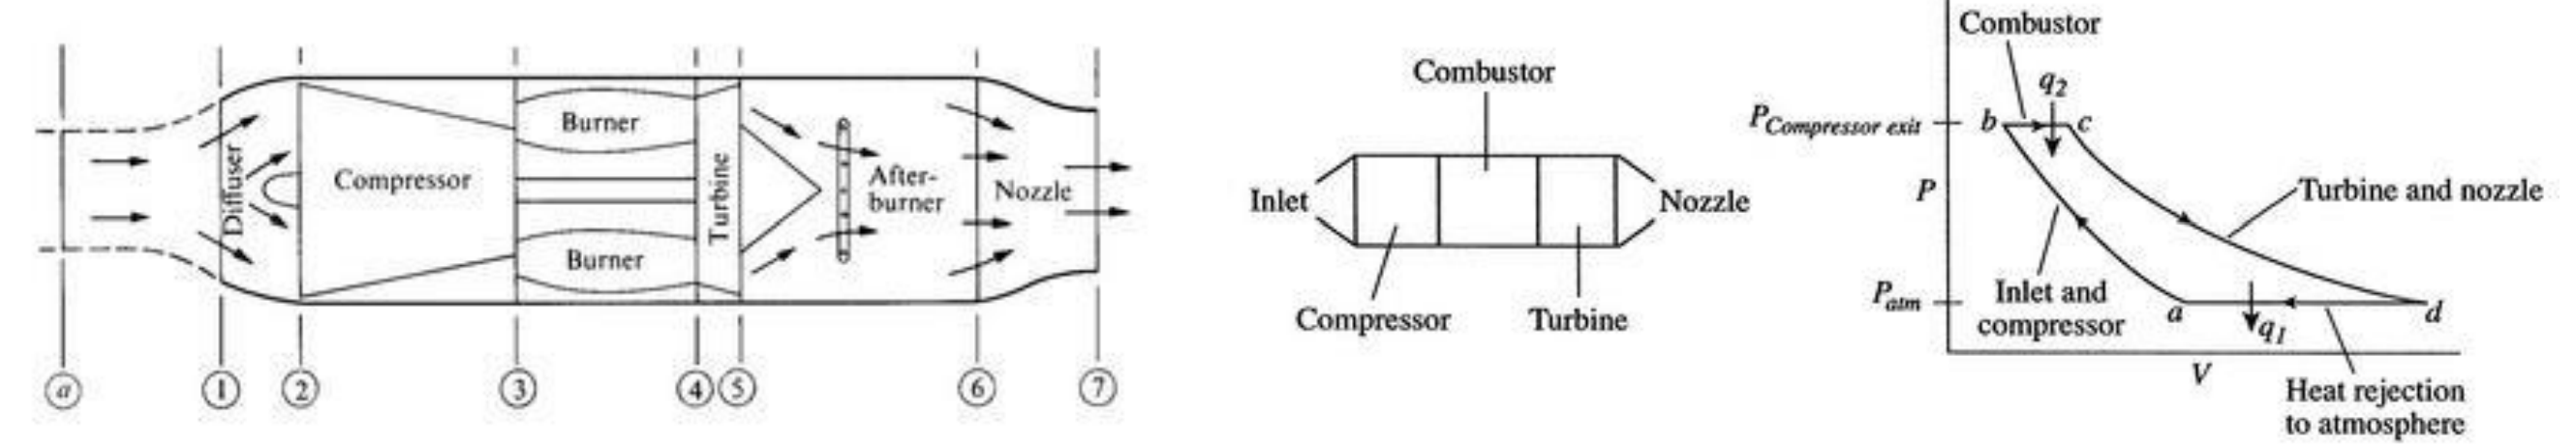
\includegraphics[width = \textwidth]{img/figure20.png}
    \caption{Brayton (or Joule) cycle.}
\end{figure}
\begin{itemize}
    \item a-b: adiabatic, quasi-static (or reversible) compression in the inlet and compressor
    \item b-c: constant pressure fuel combustion (idealised as constant pressure heat addition)
    \item c-d: adiabatic, quasi-static (or reversible) expansion in the turbine and exhaust nozzle, with which we take some work out of the air and use it to drive the compressor and take the remaining work out and use it to accelerate fluid for jet propulsion, or to turn a generator for electrical power generation
    \item d-a: cool the air at constant pressure back to its initial condition
\end{itemize}
\begin{itemize}
    \item \textbf{Fan} - the large spinning fan sucks in large quantities of air. It then speeds this air up and splits it into two parts. One part continues through the ``core'' or centre of the engine, where it is acted upon by the other engine components. The second part ``bypasses'' the core of the engine. It goes through a duct that surrounds the core to the back of the engine where it produces much of the force that propels the airplane forward. The cooler air helps to quiet the engine as well as adding thrust to the engine.
    \item \textbf{Compressor} - the compressor is the first component in the engine core. The compressor squeezes the air that enters it into progressively smaller areas, resulting in an increase in the air pressure. This results in an increase in the energy potential of the air. The squashed air is forced into the combustion chamber. 
    \item \textbf{Combustor} - in the combustor the air is mixed with fuel and then ignited. THis provides a high temperature, high-energy airflow. The fuel burns with the oxygen in the comrpessed air, producing hot expanding gases. The inside of the combustor is often made of ceramic materials to provide a heat-resistant chamber. The temperature can reach \SI{2700}{\degree C}
    \item \textbf{Turbine} - the high-energy airflow coming out of the combustor goes into the turbine, causing the turbine blades to rotate. The turbines are linked by a shaft to turn the blades in the compressor and spin the intake fan at the front. This rotation takes some energy from the high-energy flow that is used to drive the fan and the compressor. The gases produced in the combustion chamber move through the turbine and spin its blades. The turbines of the jet spin around thousands of times. They are on fixed shafts which have several sets of ball-bearings in between them.
    \item \textbf{Nozzle} - the nozzle produces the thrust for the plane. The energy depleted airflow that passed the turbine in addition to the colder air that bypassed the engine core, produces a force when exiting the nozzle that acts to propel the engine, and therefore the airplane, forward. The combination of the hot air and cold air are expelled and produce an exhaust, which causes a forward thrust. The nozzle may be preceded by a mixer, which combine the high temperature air coming from the engine core with the lower temperature air that was bypassed in the fan. The mixer helps to make the enginer quieter. 
\end{itemize}
\subsection{Typical values}
\begin{figure}[H]
    \centering
    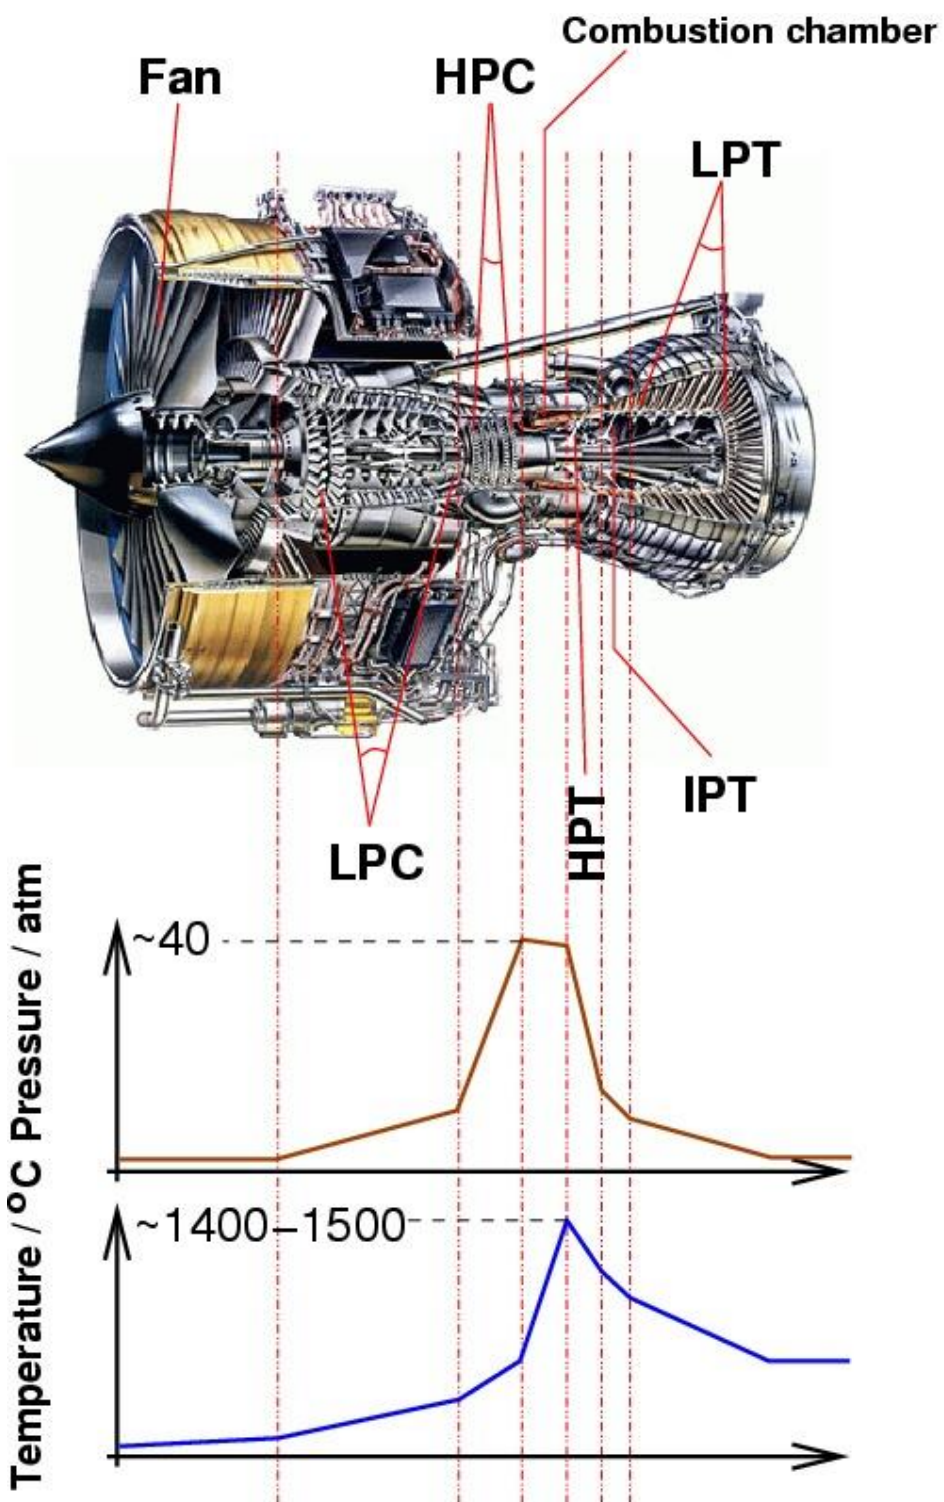
\includegraphics[width =0.5\textwidth]{img/figure21.png}
    \caption{Typical temperature values for different stages of cycle in bypass gas-turbine engine.}
\end{figure}
\begin{table}[H]
    \centering
    \begin{tabular}{@{}ll@{}}
        \toprule
        \textbf{Metal} & \textbf{Melting point}\\
        \midrule
        Titanium & \SI{1668}{\degree C}\\
        Nickel & \SI{1455}{\degree C}\\
        Steel & \SI{1370}{\degree C}\\
        \bottomrule
    \end{tabular}
    \caption{Table to show melting points of various metals used in bypass gas-turbine engines.}
\end{table}
Combustion at about 1800-\SI{1900}{\degree C}. Large centrifugal acceleration \SI{25000}{rpm} for large engines \SI{500000}{rpm} for micro gas turbine. Higher temperature makes the thermodynamic efficiency greater (about 60\%). Combustion temperature is above melting point of metals. 
\begin{table}[H]
    \centering
    \begin{tabular}{@{}ll@{}}
        \toprule
        \textbf{Fuel} & \textbf{Combustion temperature}\\
        \midrule
        Methane (in air) & \SI{1950}{\degree C}\\
        Hydrogen (in air) & \SI{2110}{\degree C}\\
        Propane (in oxygen) & \SI{2880}{\degree C}\\
        \bottomrule
    \end{tabular}
    \caption{Table to show combustion temperatures of various fuels.}
\end{table}
\subsubsection{Meeting the needs}
\begin{enumerate}
    \item Choice of material
    \item Manufacturing technique
    \item Design
\end{enumerate}
\begin{figure}[H]
    \centering
    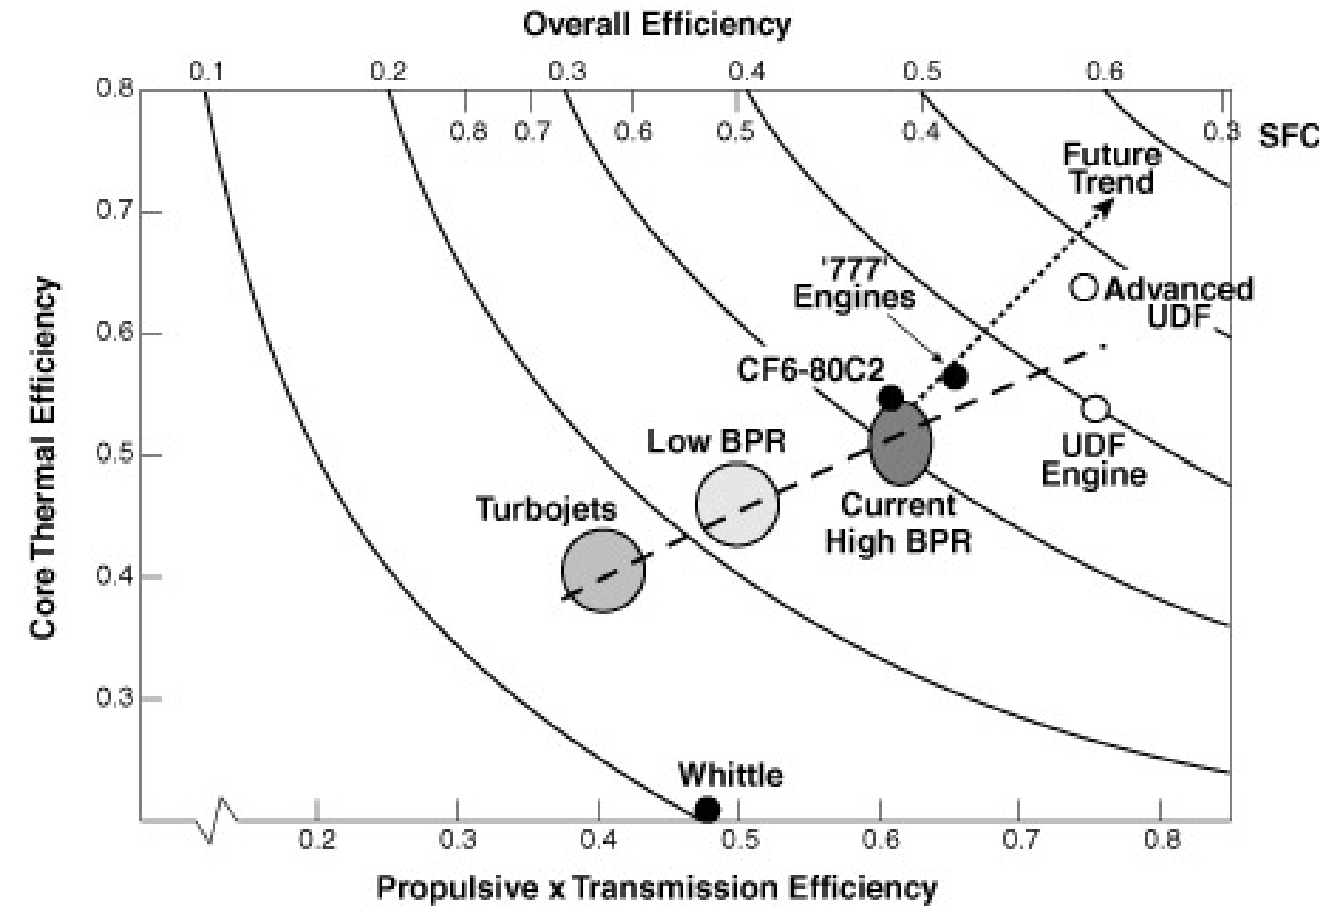
\includegraphics[width =0.8\textwidth]{img/figure22.png}
    \caption{Efficiencies of various gas-turbine engines.}
\end{figure}
\subsection{Material selection}
Considerations:
\begin{enumerate}
    \item Strength and weight: titanium
    \item Temperature: major constraint is the material selection for the hot section (combustor and turbine) of the engine
\end{enumerate}
The need for better materials spurred much research in the field of alloys and manufacturing techniques, and that research resulting in a long list of new materials and methods that make modern gas turbines possible. One of the earliest of these was Nimonic 90 (nickel-based, high-temperature, low-creep superalloys Ni 54\%, Cr 18-21\%, Co 15-21\%, Ti 2-3\%, Al 1-2\%).

The development of superalloys in the 1940s and new processing methods such as vacuum induction melting in the 1950s greatly increased the temperature capability of turbine blades. Further processing methods like hot isostatic pressing improved the alloys used for turbine blades and increased turbine blade performance. Modern turbine blades often use nickel-based superalloys that incorporate chromium, cobalt and rhenium.
\begin{figure}[H]
    \centering
    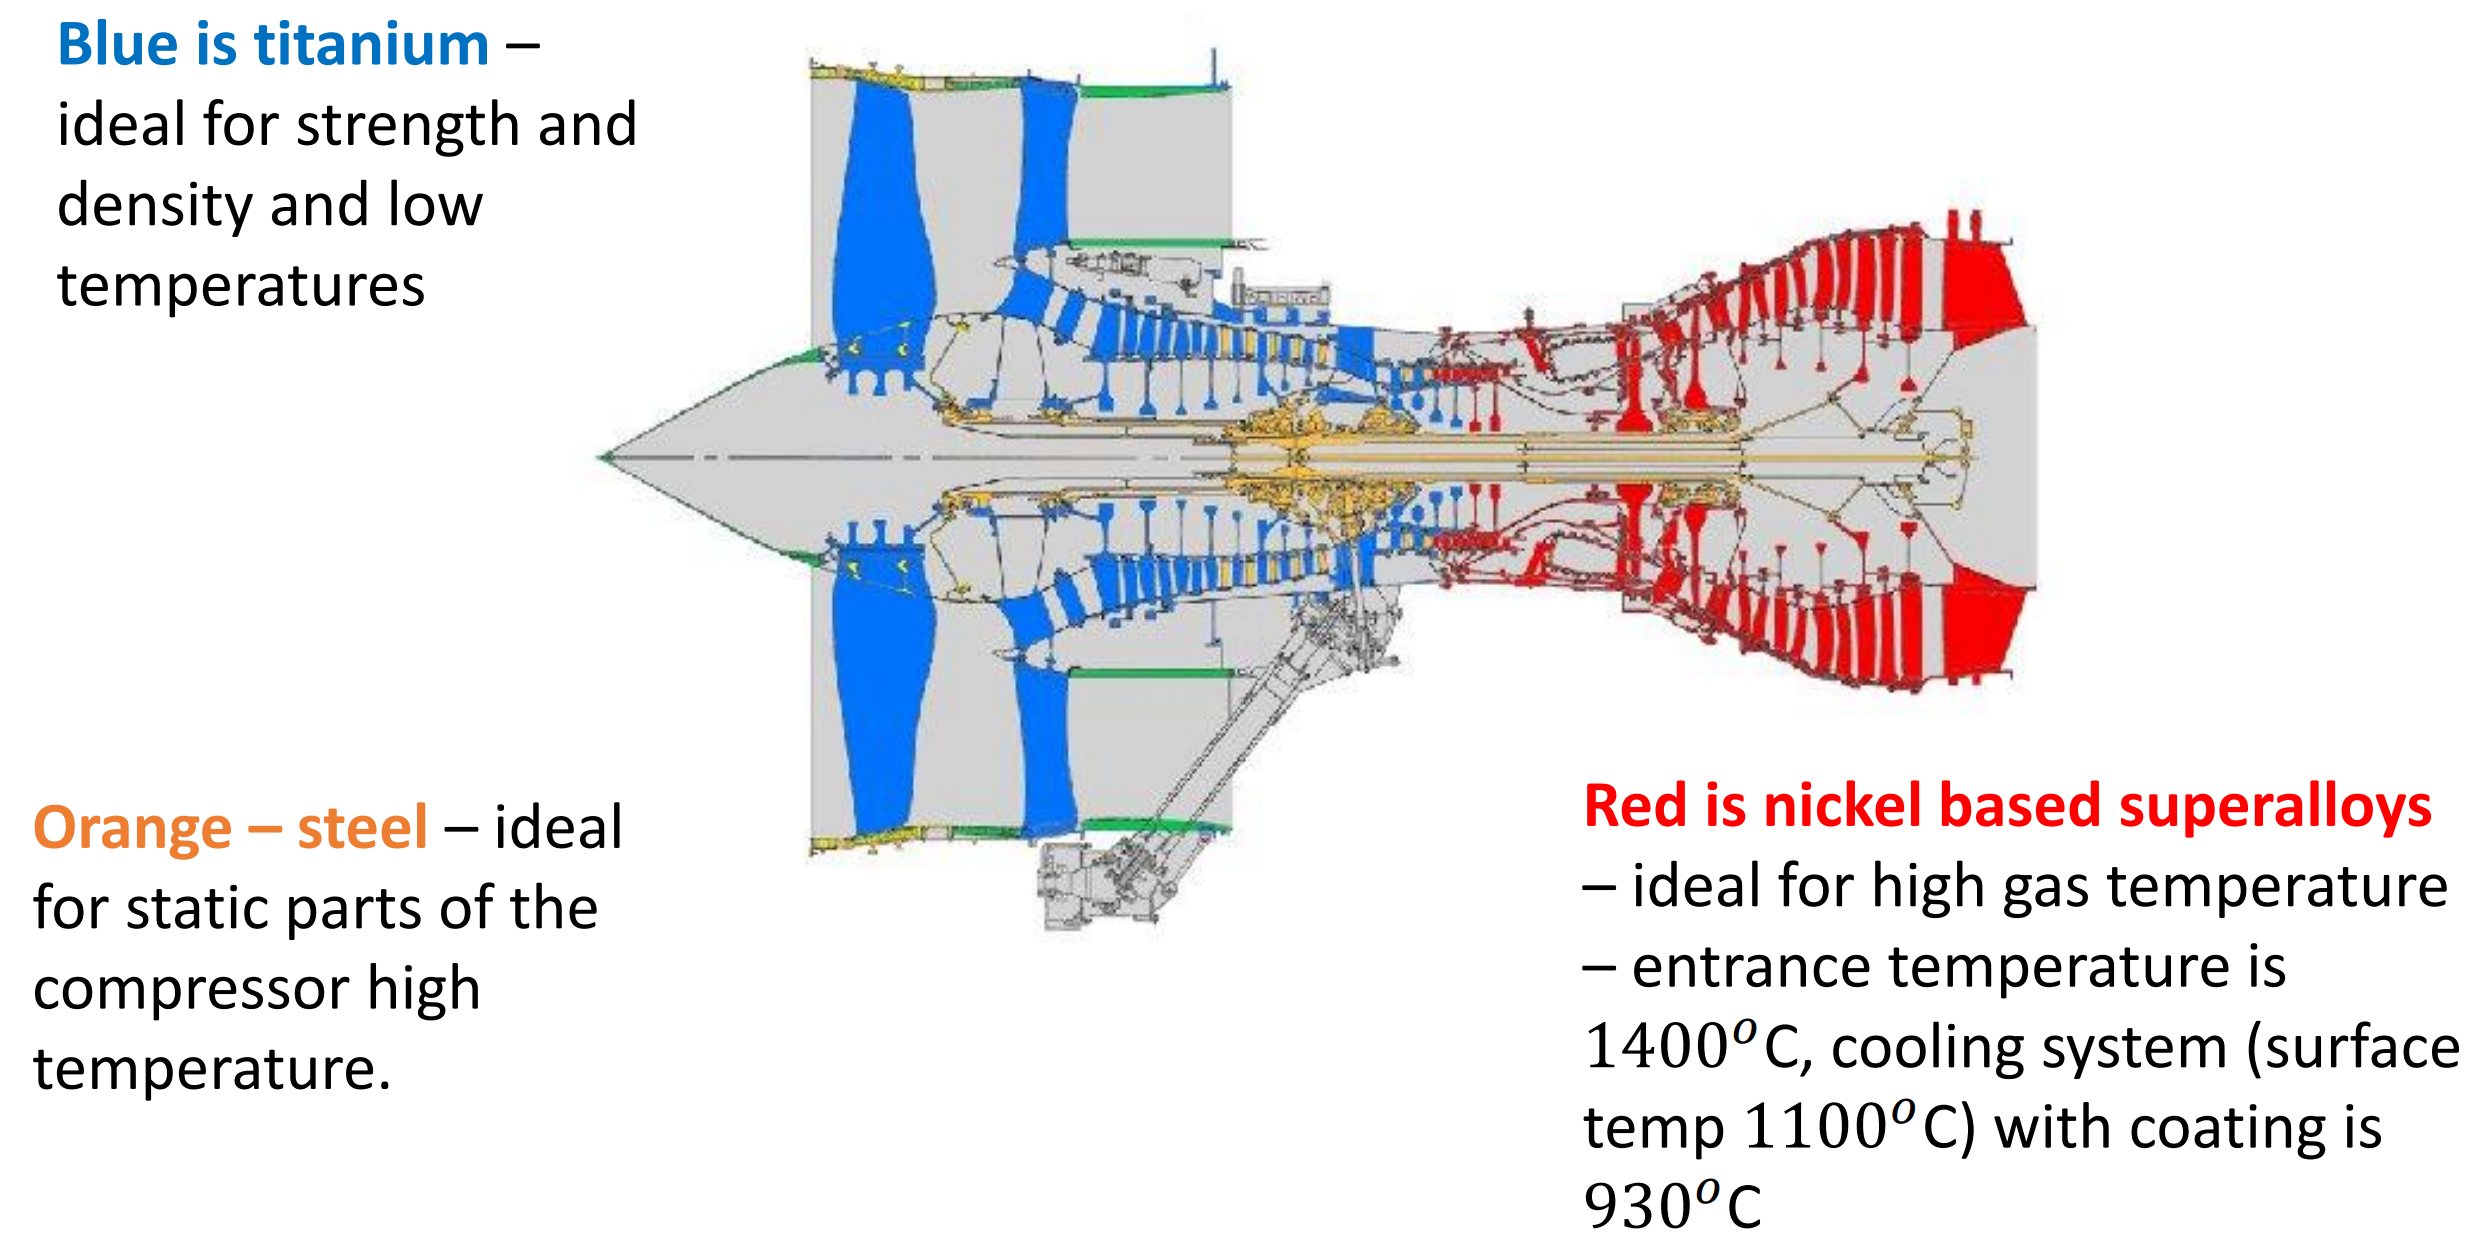
\includegraphics[width =\textwidth]{img/figure23.png}
    \caption{Usage of different alloys within the engine.}
\end{figure}
\begin{figure}[H]
    \centering
    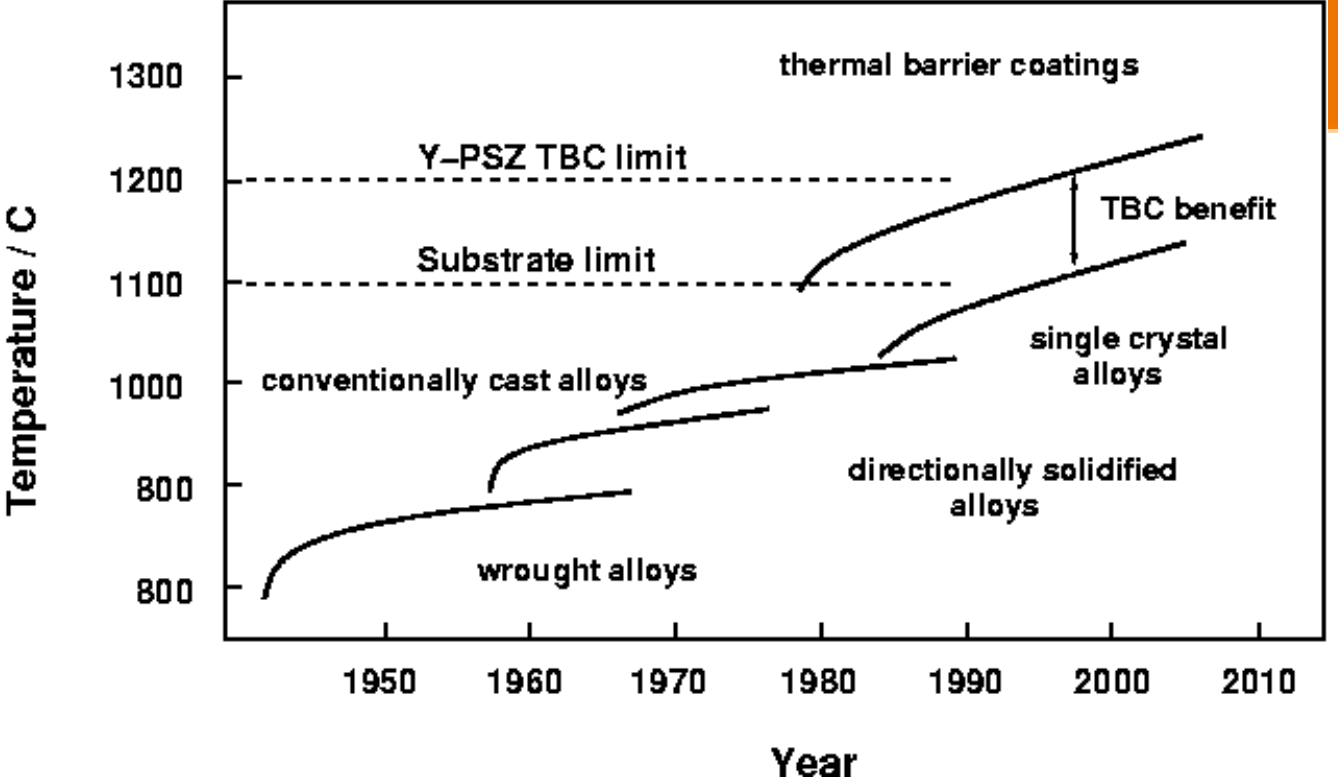
\includegraphics[width =0.8\textwidth]{img/figure24.png}
    \caption{Development of alloys.}
\end{figure}
Titanium - good for weight and strength (poor with heat).

Alloy improvement, directional and single-crystal solidifcation have contributed significantly, but arguably, the empahsis has been shifted to coating systems which have allowed an increase of gas temperatures up to \SI{1100}{\degree C}. Coatings in gas turbines serve a variety of purposes. A first requirement to operate turbines at higher temperatures was, of course, improved strength. Unfortunately, these conditions also mean severe oxidation / corrosion problems, and to make things worse, the improvement in mechanical properties of the base alloys was made at the expense of environmental resistance. 

The first purpose of coatings was to improve poor oxidation resistance of the base alloy (aluminide, Pt-aluminide, MCrAlY). A second type of coatings applied to high-temperature parts are known as thermal barrier coatings (TBC). These are ceramic coatings with very low thermal conductivity and thin (\SI{200}{\micro\meter}). Drop of 100-\SI{300}{\degree C} between the gas and metal surface temperatures but are `oxygen transparent' and do not prevent oxidation of the underlying substrate.
\subsection{Manufacturing process}
Aside from the alloy improvements, a major breakthrough was the development of directional solidification (DS) and single crystal (SC) production methods. These methods help greatly increase strength against fatigue and creep by aligning grain boundaries in one direction (DS) or by eliminating grain boundaries altogether (SC).

Recent generations of superalloys for single crystal turbine blades contain relatively high percentages of refractory elements such as Ta, W or Re which enhance the high-temperature mechanical properties. 

This is done at the expense of Cr and Al. Given the severe environmental conditions in which the blades operate, the removal of the elements (beneficical for oxidation resistance) implies even greater degradation problems. 

To reduce the oxidation corrosion resistance, an external coating is applied to the blades. Its purpose is to allow for the growth of a resistant oxide layer. Of all possible oxides $\alpha$-Al$_2$O$_3$ offers excellent protection and very low growth rates (in a minority of cases, Cr oxides are preferred). The composition of the coating must therefore be chosen carefulyl so as to ensure growth of $\alpha$-Al$_2$O$_3$.
\begin{figure}[H]
    \centering
    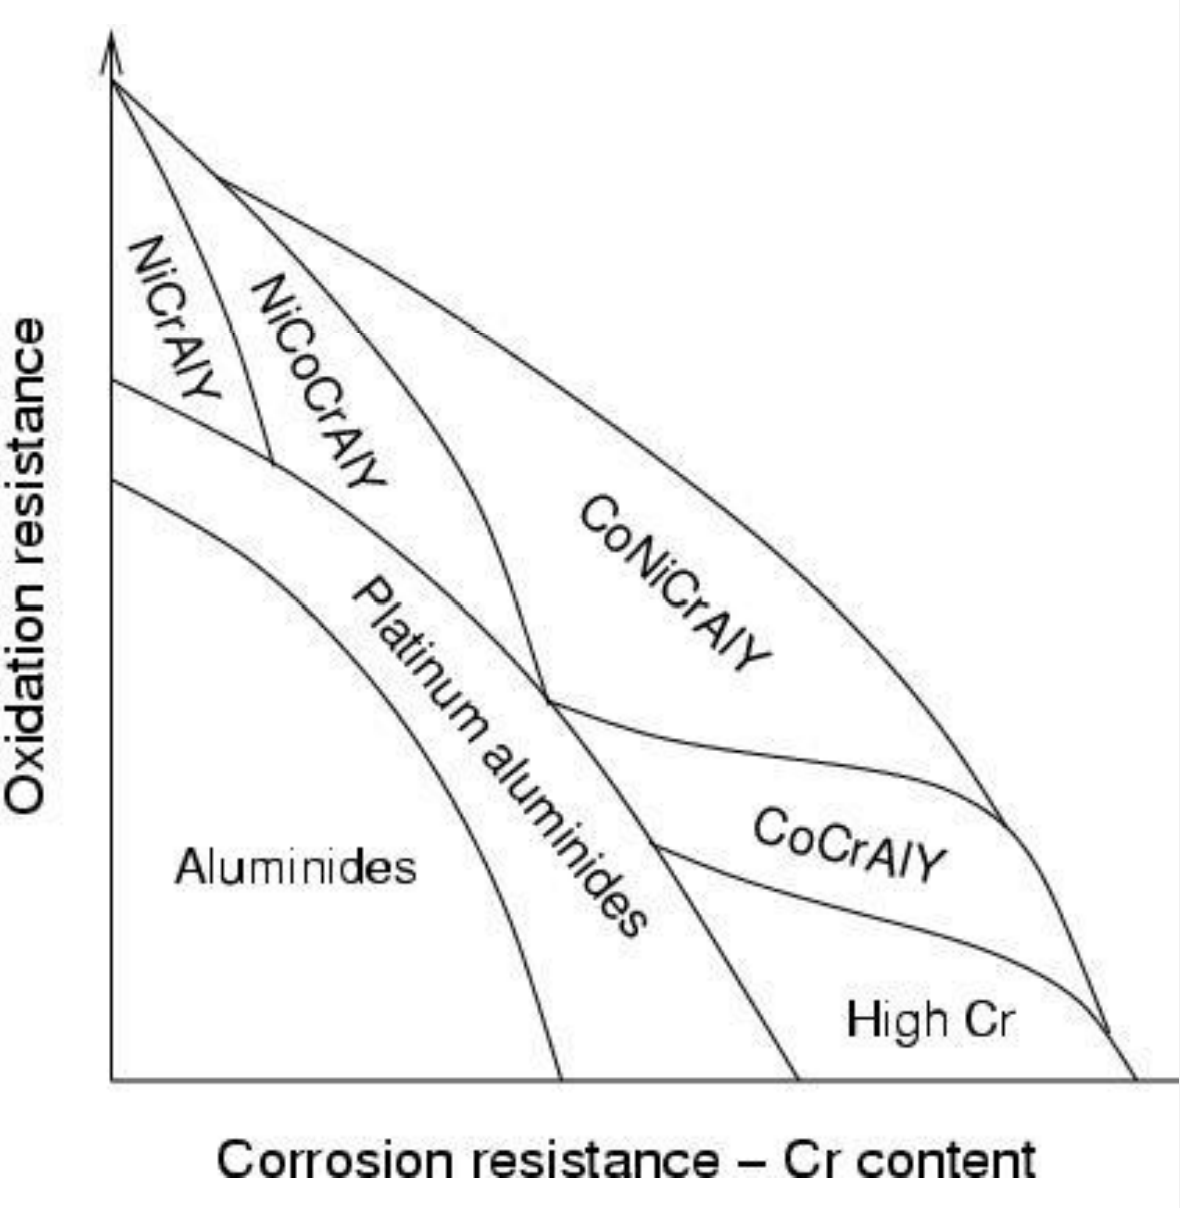
\includegraphics[width =0.6\textwidth]{img/figure25.png}
    \caption{Oxidation and corrosion resistance of different alloys.}
\end{figure}
\begin{figure}[H]
    \centering
    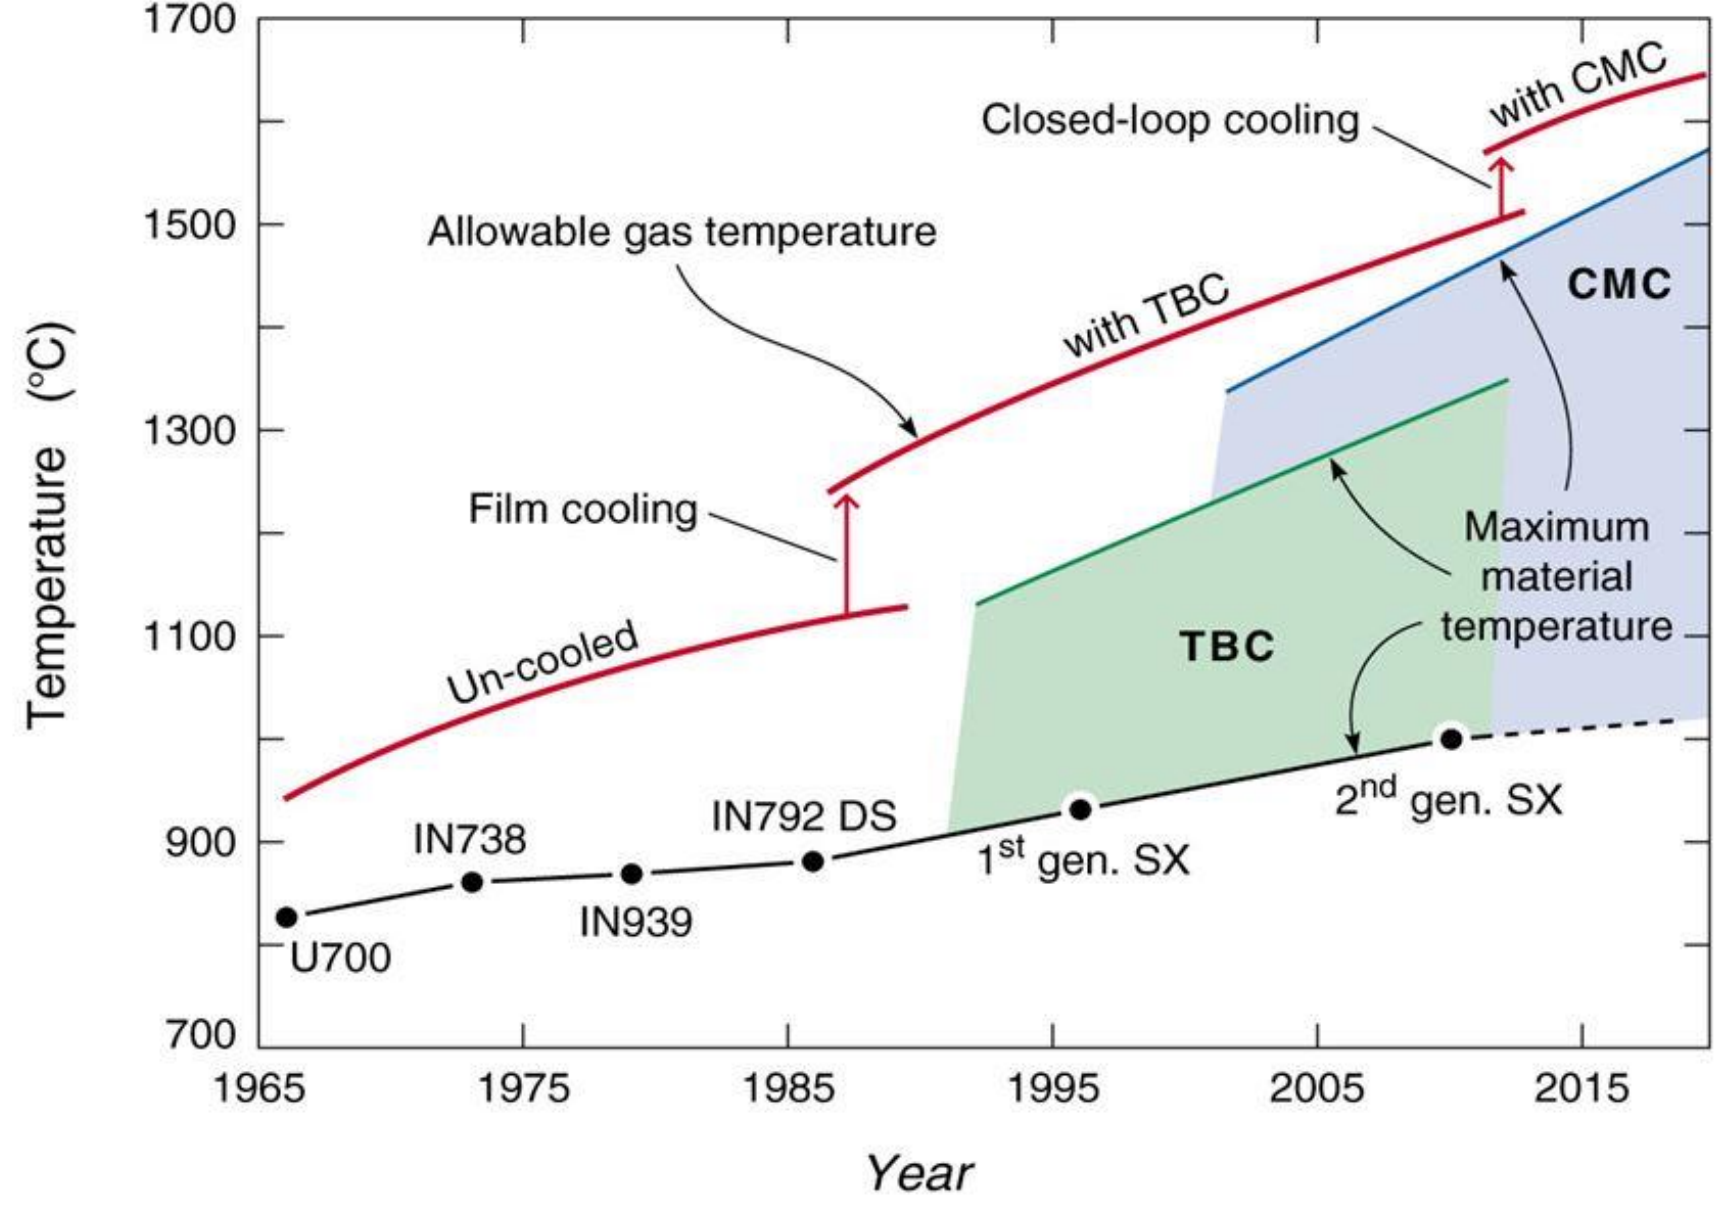
\includegraphics[width =0.8\textwidth]{img/figure26.png}
    \caption{Temperature resistance of TBCs and CMCs over the years.}
\end{figure}
TBC - thermal barrier coating. CMC - ceramic matrix composite.
\subsection{Thermal barrier coating}
Thermal barrier coatings (TBC) are advanced materials systems usually applied to metallic surfaces, such as on gas turbine or aero-engine parts, operating at elevated temperatures, as a form of exhaust heat management. These \SI{100}{\micro\meter} to \SI{2}{mm} coatings serve to insulate components from large and prolonged heat loads by utilising thermally insulating materials which can sustain an appreciable temperature difference between the load-bearing alloys and the coating surface.
\begin{figure}[H]
    \centering
    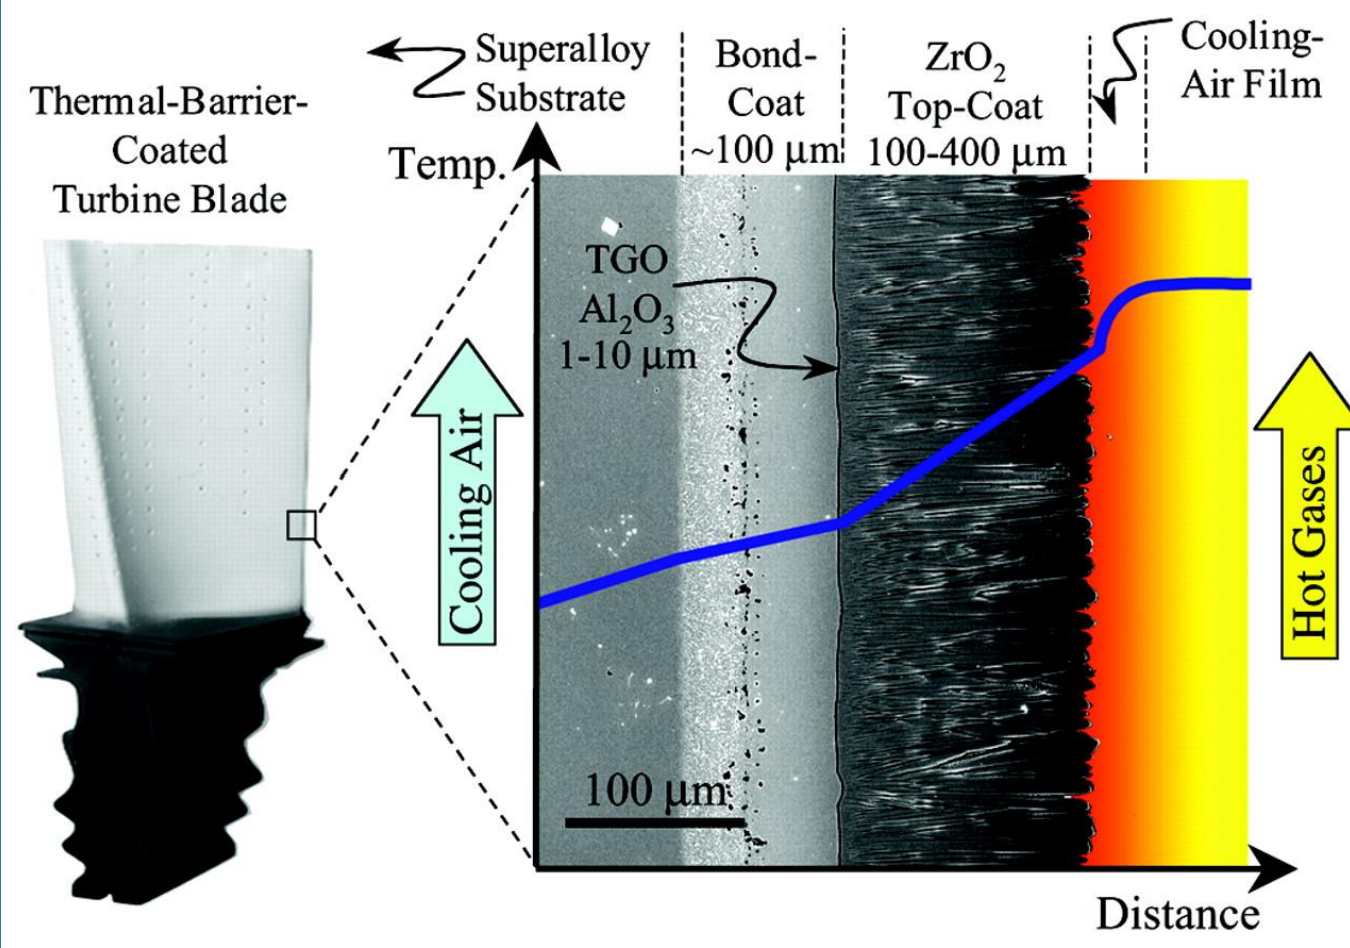
\includegraphics[width =0.6\textwidth]{img/figure27.png}
    \caption{Thermal barrier coatings (TBCs).}
\end{figure}
Four layers:
\begin{enumerate}
    \item The metal substrate
    \item Metallic bond coat
    \item Thermally-grown oxide (TGO)
    \item Ceramic topcoat. The ceramic topcoat is typically composed of yttria-stabilised zirconia (YSZ) which is desirable for having very low of conductivity while remaining stable at nominal operating temperatures typically seen in applications. This ceramic layer creates the largest thermal gradient of the TBC and keeps the lower layers at a lower temperature than the surface.
\end{enumerate}
\begin{figure}[H]
    \centering
    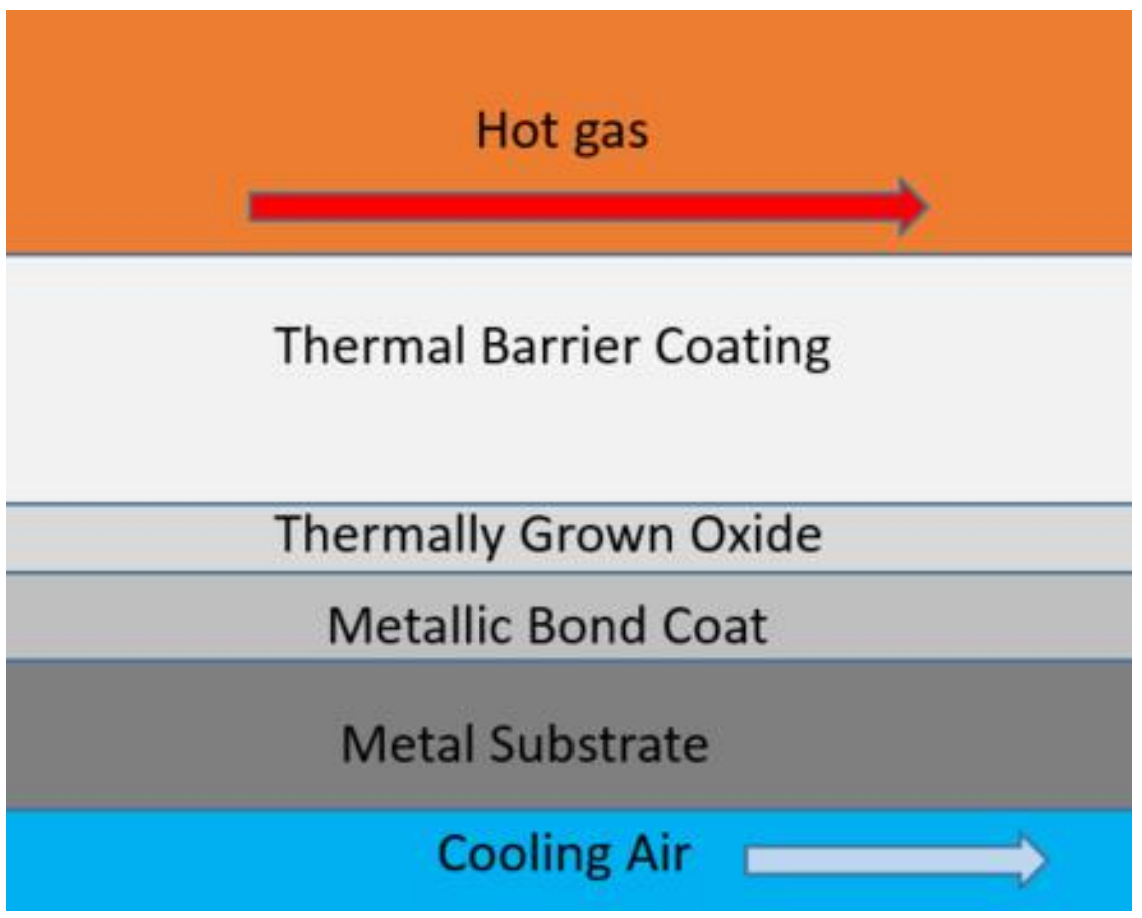
\includegraphics[width =0.6\textwidth]{img/figure28.png}
    \caption{Thermal barrier coating composition.}
\end{figure}
TBCs improved corrosion and oxidation resistance, both which became greater concerns as temperatures increased. First TBCs (1970s) were aluminide coatings. Ceramic coatings in 1980s which decreased turbine blade temperature by about \SI{90}{\degree C}, improve blade life, almost doubling the life of turbine blades in some cases.
\chapter{Large Spatial and Temporal Variations of Temperature}
\section{Introduction}
Many different engineering materials are subject to intense heating and cooling in localised regions. As with our previous discussion about materials, the temperature might be spatially or temporally variable. In Lecture 13, we looked at the thermoelastic response of materials subject to small temperature variations. Their response can be dealt with via a linear elastic model. In this chapter, we look at the effect of a large temperature applied to a material which are sufficient to generate a plastic response and how the spatial and temporal variation affects the material properties.

The incandescent light build initially failed due to the thermal fatigue and melting problems. This was largely a material selection and corrosion problem. Turning a light on and off generates enormous thermal stresses, but keeping it on continuously is fine. The filament is made of tungsten which has a high melting point. The inert gases around the filament stop evaporation. Most of energy dissipated is thermal.
\subsubsection{Types of heating processes}
\begin{itemize}
    \item \textbf{Mechanical heating}, usually by friction
    \item \textbf{Electrical heating}, using the material itself for energy release (e.g. induction heating), or more commonly by external means with an electrical resistance made of Nichrome (60\% Ni, 25\% Fe, 15\% Cr) or Kanthal (70\%, 24\% Cr, 5\% Al)
    \item \textbf{Radiation heating}, either with microwaves, infrared radiation from heated wires protected inside a quartz-glass (wires can be made of tungsten, carbon, Kanthal or Nichrome; naked Nichrome coiled wire was also used in the past), or using visible radiation (with a laser).
    \item \textbf{Chemical heating}, mainly by combustion, but also by hydrogen formation after atomic hydrogen is produced in an electric car, for instance.
    \item \textbf{Nuclear heating}, by nuclear fission or fusion
\end{itemize}
\begin{figure}[H]
    \centering
    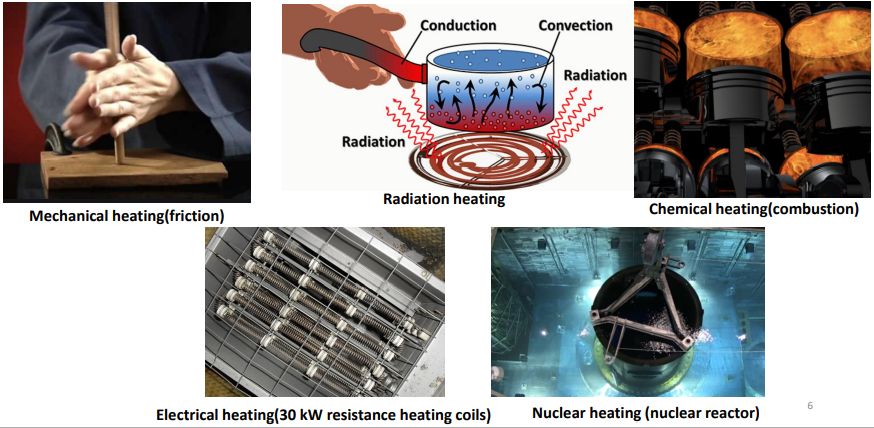
\includegraphics[width = 0.8\textwidth]{img/figure41.png}
    \caption{Heating processes.}
\end{figure}
\begin{figure}[H]
    \centering
    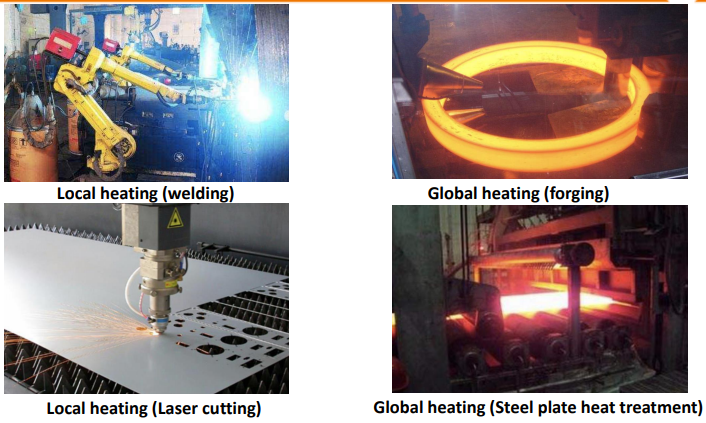
\includegraphics[width = 0.8\textwidth]{img/figure40.png}
    \caption{Localised heating processes.}
\end{figure}
\section{Practical application of heat to a material}
Any time a material is heated, the heat is applied spatially and temporally. The characteristics scales have quite different effects on the material and structure.
\begin{table}[H]
    \centering
    \begin{tabular}{@{}lll@{}}
        \toprule
             & \textbf{Localised} & \textbf{Uniform} \\
        \midrule
        Slow & Welding            & Heat treatment   \\
        Fast & Thermal shocking   & Quenching        \\
        \bottomrule
    \end{tabular}
    \caption{Spatial and temporal heat application.}
\end{table}
\subsection{Welding}
\begin{itemize}
    \item TIG - Tungsten gas - electrode is tungsten. You do not need a metal filter. Need a gas tank to protect the weld - most often applied to stainless steels and light metals
    \item Flux-cored Arc Welding - similar to MIG. Uses a wire to serve as an electrode and a metal filler fed through the wand. Wire has a flux that creates the gas shield. Tends to have slag left so usually needs a clean-up
    \item Stick (Shielded Metal Arc Welding). Replaceable electrode stick t hat forms the filler metal. Arc is created at the end of the electrode. Stick is coated in flux that protects the metal from oxidation
    \item MIG welding (metal inert gas). Filler metal is consumable wire that acts as an electrode
    \item Laser beam welding - used on a few metals with laser providing the heat
    \item Plasma Arc Welding - uses a smaller arc with a high pressurised gas that is ionised and electrically conductive
\end{itemize}
Small amount of molten metal are introduced in the gap between two components to solidify the body. Major regions are:
\begin{enumerate}
    \item Fusion where the parts of the metal have melted and combined with filler material
    \item Heat affected zone - region next to steel that have undergone microstructural changes
\end{enumerate}
\subsection{Friction welding}
\url{https://www.youtube.com/watch?v=RTEP9QdTn5k}
\begin{figure}[H]
    \centering
    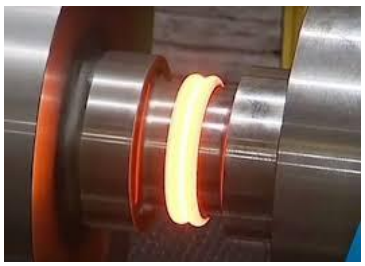
\includegraphics[width = 0.8\textwidth]{img/figure44.png}
    \caption{Friction welding.}
\end{figure}
\subsection{Radiation heating}
\begin{figure}[H]
    \centering
    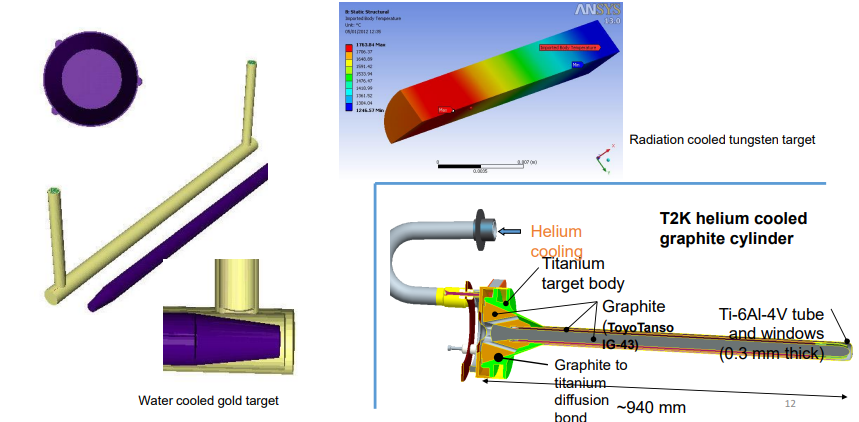
\includegraphics[width = 0.8\textwidth]{img/figure42.png}
    \caption{Radiation heating.}
\end{figure}
\subsection{Laser heating}
\begin{figure}[H]
    \centering
    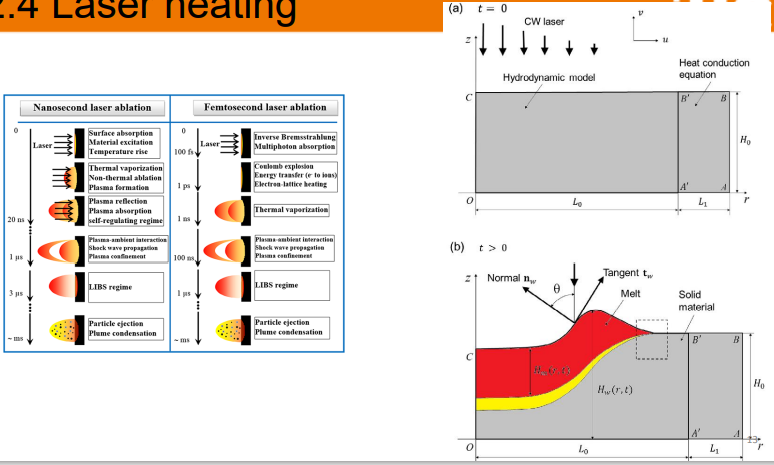
\includegraphics[width = 0.8\textwidth]{img/figure45.png}
    \caption{Laser heating.}
\end{figure}
\begin{figure}[H]
    \centering
    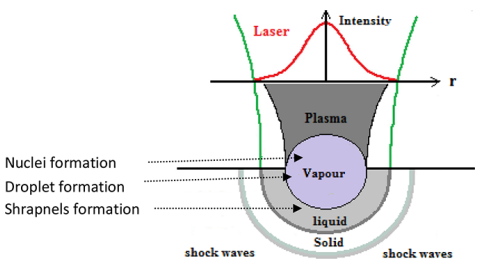
\includegraphics[width = 0.8\textwidth]{img/figure46.png}
    \caption{Close-up of laser heating.}
\end{figure}
\begin{figure}[H]
    \centering
    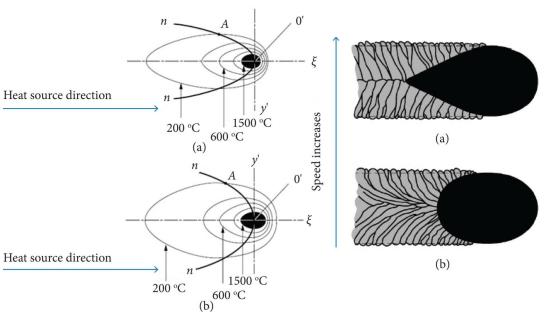
\includegraphics[width = 0.8\textwidth]{img/figure47.png}
    \caption{Close-up of laser heating.}
\end{figure}
The heat spreads out through diffusion from a moving source. The temperature distribution can be analysed using simple mathematical models of a moving source and this is discussed in Worksheet 15.
\section{Structural changes in the matter}
\url{https://www.youtube.com/watch?v=uG35D_euM-0&authuser=0}
\subsection{Microstructural changes}
Metals are comprised of a symmetrical structure of atoms known as an allotrope. Heating the metal will displace atoms from their position and the displaced atoms form a new structure. This process is known as allotropic phase transformation. Allotropic phase transformation alters the hardness, strength and ductility of the metal. The most important allotropic phase transformation is undergone by iron. When iron is heated past \SI{912}{\degree C} it is able to absorb more carbon which is essential for the manufacture of stainless steel.
\begin{figure}[H]
    \centering
    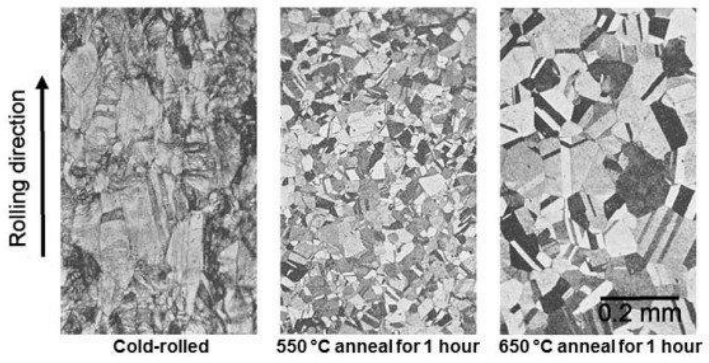
\includegraphics[width = 0.8\textwidth]{img/figure43.png}
    \caption{Effect on microstructure from cold rolling and then annealing.}
\end{figure}
\subsubsection{Heat treatment}
\textbf{Annealing} is used to soften metals including iron, steel, copper, brass and silver. The process involves heating the metal to a specific temperature then allowing it to cool slowly at a controlled rate. Annealing alters the physical and chemical properties of the metal to increase ductility and reduce hardness. This facilitates shaping, stamping or forming processes, and allows the metal to be cut more easily. Annealing also enhances electrical conductivity.

\textbf{Normalising} is applied to alloys to provide uniformity in grain size and composition. The metal is heated to a predefined temperature then cooled by air. The resulting metal is free of undesirable impurities and exhibits greater strength and hardness. Normalising is often used to produce a harder and stronger steel, albeit one that is less ductile than that produced by annealing. Typically, the normalising process is performed on materials that will be subjected to machining, because the process has improved this attribute.

\textbf{Hardening} is applied to steel and other alloys to improve their mechanical properties. During hardening, the metal is heated at a high temperature and this temperature is maintained until a proportion of carbon has been dissolved. Next the metal will is quenched, which involves rapidly cooling it in oil or water. Hardening will produce an alloy which has high strength and and wear resistance. However, hardening will also increase brittleness and is not suitable for engineering applications. When there is a need to have the surface of the component hard enough to resist wear and erosion, while maintaining ductility and toughness to withstand impact and shock loading - surface hardening would be used.

\textbf{Tempering} is applied to steel where ductility is desired. Untempered steel is very hard but too brittle for most practical applications. Tempering is a low temperature heat treatment process normally performed after hardening (neutral hardening, double hardening, atmospheric carburising, carbonitriding, or induction hardening) in order to reach a desired hardness/toughness ratio. the process involves heating steel to a lower temperature to reduce some of the excess hardness. The metal is then allowed to cool in still air which results in a tougher and less brittle steel.
\subsection{Macroscopic changes}
Large temperature variations lead to inelastic and non-recoverable deformations. For plastic deformation require about 0.2\% residual strain. Since the strain generated a temperature difference of $\Delta T$ scales as $\epsilon \sim \Delta T \alpha$. With a typical value of a $\alpha \sim \SI{1e-5}{\per\kelvin}$, we only need $\Delta T \sim \SI{200}{\kelvin}$ to generate this strain. Large temperatures leads to melting, rearrangement of bonds and this is what is used in casting and welding. Ductile and malleable materials can absorb changes while brittle materials fracture.
\section{Soldering, brazing, welding}
\begin{itemize}
    \item Soldering is a low-temperature process (60-\SI{400}{\degree C}) that uses a low-melting metal (a base of tin combined with lead, silver, antimony, bismuth, indium) to join similar or dissimilar metals; it is mainly used in electronic boards
    \item Brazing is a mid-temperature process (450-\SI{1200}{\degree C}) that uses a high-melting metal (a base of silver combined with nickel, copper, zinc) to join similar or dissimilar metals; it is mainly used in copper piping and jewellery
    \item Welding is a high temperature process (800-\SI{2000}{\degree C}) that uses a powerful heat source to locally melt and join similar metals; it is mainly used in iron and steel work
\end{itemize}
\subsubsection{Influence of localised heating}
Close to the weld there is a heat affected region where the microstructure is affected by the heat. The metal in this area is generally weaker than the base material and the fusion zone. This is where the residual stresses are found.
\begin{figure}[H]
    \centering
    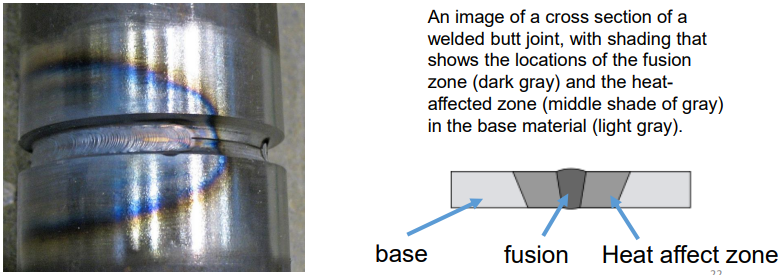
\includegraphics[width = 0.8\textwidth]{img/figure48.png}
    \caption{Influence of localised heating on a weld.}
\end{figure}
\subsubsection{Heat affected zone}
This is the ring that surrounds the weld which affects the alloy. If thermal diffusivity is high, cooling rate is high so the HAZ is smaller. If thermal diffusivity is low, cooling rate is low so the HAZ is bigger. Other measures are used, such as rate of heat input for weld where:
\begin{equation}
    Q = \frac{60VI}{1000U}\times \textrm{efficiency}
\end{equation}
\begin{itemize}
    \item $Q$ is the heat input (\si{\kilo\joule\per\milli\meter})
    \item $VI$ is the electrical power
    \item $U$ is the speed of the weld
\end{itemize}
Usually we need $Q \approx 10-\SI{25}{\kilo\joule\per\milli\meter}$.
\begin{table}[H]
    \centering
    \begin{tabular}{@{}ll@{}}
        \toprule
        \textbf{Weld} & \textbf{Efficiency} \\
        \midrule
        PAW           & 0.46                \\
        GTAW          & 0.65                \\
        Gas metal arc & 0.83                \\
        \bottomrule
    \end{tabular}
    \caption{Welding efficiencies.}
\end{table}
\subsubsection{Thermoplastic shrinkage}
When a plate is heated, there is an elastic convex deformation that fades as it is cooled and a plastic concave deformation. This is exploited in ship manufacturing techniques to create curved sheets.
\begin{figure}[H]
    \centering
    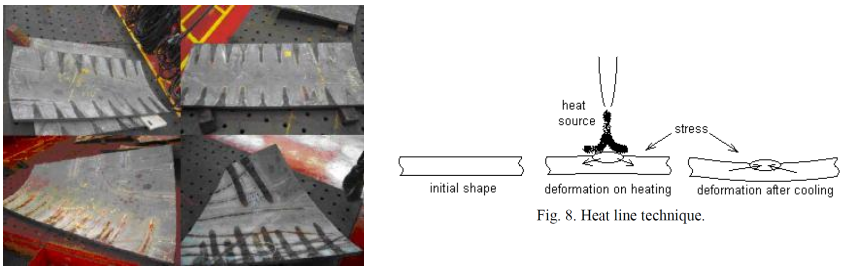
\includegraphics[width = 0.8\textwidth]{img/figure49.png}
    \caption{Thermoplastic shrinkage.}
\end{figure}
\begin{figure}[H]
    \centering
    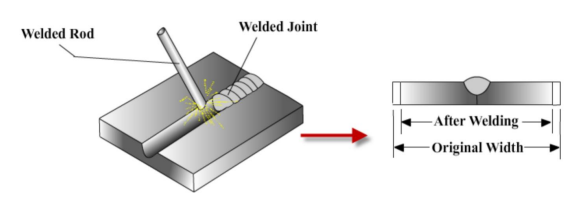
\includegraphics[width = 0.8\textwidth]{img/figure50.png}
    \caption{Weld shrinkage.}
\end{figure}
Weld shrinkage - generated by localised stresses caused by heating and distortion of the heated material. Usually leads to transverse and longitudinal shrinkage.
\subsubsection{Process of plate heating}
The process is known as heat line technique or line heating method of plate bending; it is applied mainly to mild-steel plates, and was started in the 1970s in shipbuilding. It consists of the following steps.
\begin{enumerate}
    \item Initial heating. It forces the heated mass to expand against the rest of the material, creating great stresses and a very small convex elastic deformation due to the temperature gradient
    \item High heating. Up to \SI{1200}{\kelvin} (but usually limited to $<$\SI{995}{\kelvin} to avoid the mild-steel phase transition). It lowers the strength of the heated mass so much, that plastic-yield takes place, that the side material forces the heated mass to bulge in the hottest region
    \item After cooling. Forced cooling (usually by water) increases the temperature gradient that forces the heated mass to recover its original strength but not its original shape, because the plastic deformation is not reversible, causing a shrinkage that pulls in from the rest of the material (i.e. in the whole it is not a thermal push but a thermal pull), causing a concave bending (and perhaps some cracks), and minor in-plane deformations due to the point-wise application (instead of the whole line at a time).
\end{enumerate}
\begin{figure}[H]
    \centering
    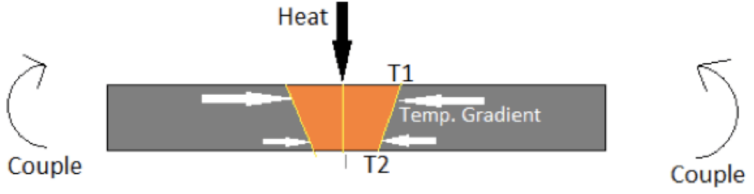
\includegraphics[width = 0.8\textwidth]{img/figure51.png}
    \caption{Plate heating.}
\end{figure}
\chapter{Low temperature environments}
\section{Introduction}
\begin{itemize}
    \item Low temperature: \SI{-273}{\degree C}, \SI{-150}{\degree C}
    \item Mechanical challenges - rapid heating / increasing gas pressure
          \begin{itemize}
              \item Failure / fatigue
          \end{itemize}
    \item Most low temperature - rise at atmospheric pressure
          \begin{itemize}
              \item Small volumes
          \end{itemize}
    \item Through design - challenge becomes managing the thermal component not the mechanical
    \item Health \& Safety - dense / cold gas moves quickly and can suffocate people
\end{itemize}
\begin{table}[H]
    \centering
    \begin{tabular}{@{}ll@{}}
        \toprule
        \textbf{Gas} & \textbf{Freezing temperature}      \\
        \midrule
        \ce{CO2}     & \SI{-78.5}{\degree C} (sublimates) \\
        Nitrogen     & \SI{-196}{\degree C}               \\
        LNG          & \SI{-161.5}{\degree C}             \\
        \bottomrule
    \end{tabular}
    \caption{Freezing temperatures of various gases.}
\end{table}
The energy density of LNG is comparable to propane and ethanol but is only 60 percent that of diesel and 70 percent that of gasoline.
\begin{figure}[H]
    \centering
    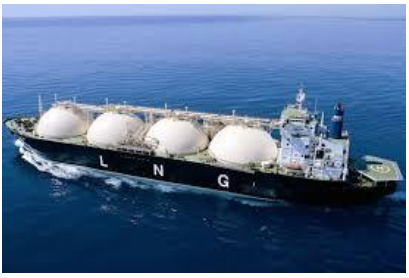
\includegraphics[width = 0.5 \textwidth]{img/figure56.png}
    \caption{LNG carrier.}
\end{figure}
An LNG carrier is a tank ship designed for transporting liquefied natural gas. At the end of 2016, the global LNG shipping fleet consisted of 439 vessels. Majority of ships have a capacity of \SI{120000}{}-\SI{140000}{\meter\cubed}.
\begin{table}[H]
    \centering
    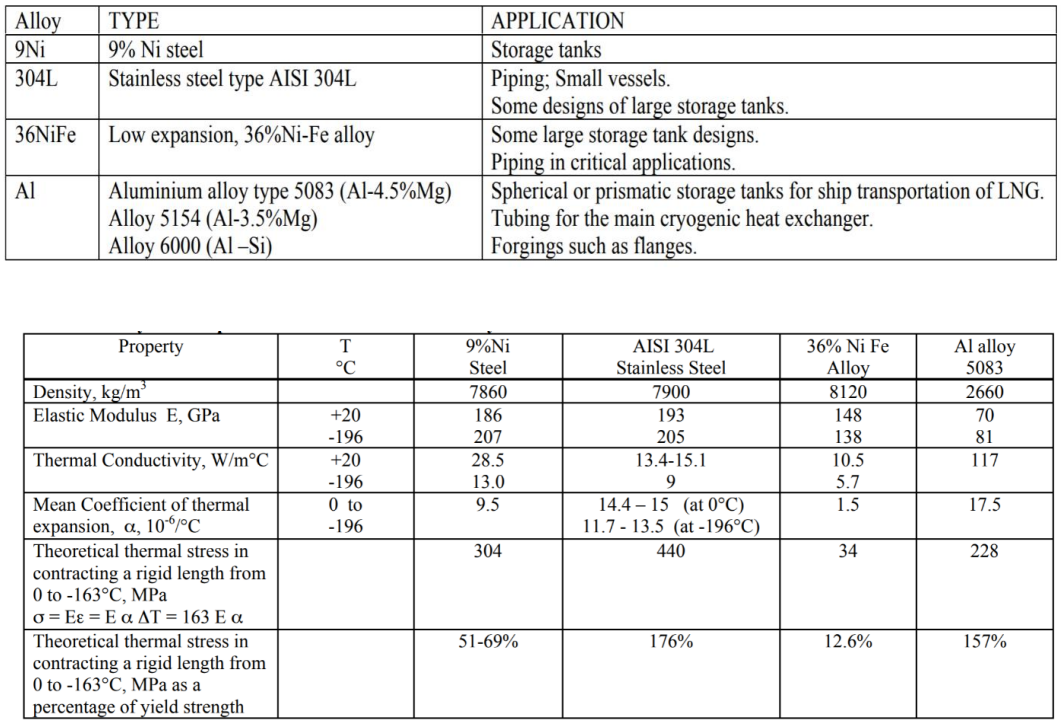
\includegraphics[width = \textwidth]{img/figure57.png}
    \caption{Tables to show material properties of storage tanks.}
\end{table}
\begin{table}[H]
    \centering
    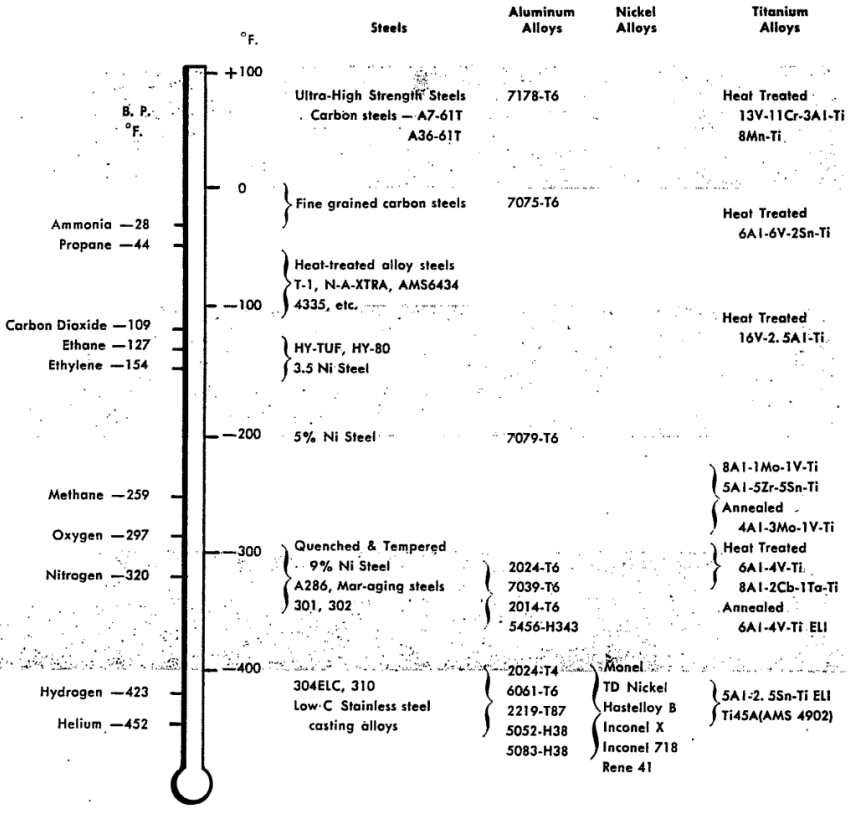
\includegraphics[width = \textwidth]{img/figure58.png}
    \caption{Table to show materials used to store different low temperature materials.}
\end{table}
\section{Engineering applications}
\subsection{LNG - liquefied natural gas}
Methane, \ce{CH4} (with some ethane). 1/6000$^{\textrm{th}}$ the volume of natural gas in the gaseous state (at standard condition for temperature and pressure). It is odourless, colourless, non-toxic and non-corrosive. Hazards include flammability after vaporisation into a gaseous state, freezing and asphyxia. The liquefaction process involves removal of certain components, such as dust, acid gases, helium, water and heavy hydrocarbons, which could cause difficulty downstream. The natural gas is then condensed into a liquid at close to atmospheric pressure by cooling it to approximately \SI{-162}{\degree C}. Maximum transport pressure is set at around \SI{25}{\kilo\pascal}.
\subsection{Cryogenic transport}
Transfer lines are a form of cryostat. Used to transport cryogenic fluids between cryogenic devices. Simplest form is a vacuum jacketed pipe connecting two flasks. Heat is absorbed by the liquid (nitrogen) and as the pipe gets longer, more heating occurs and more vapour generated (which is lost). Higher pressure differential, more heating occurs. The most important design elements are:
\begin{itemize}
    \item Geometry
    \item Mass flow rate
    \item Temperature and pressure change
    \item Cryogenic fluid
    \item Mechanical properties of the materials
\end{itemize}
\section{Thermal bowing}
\begin{figure}[H]
    \centering
    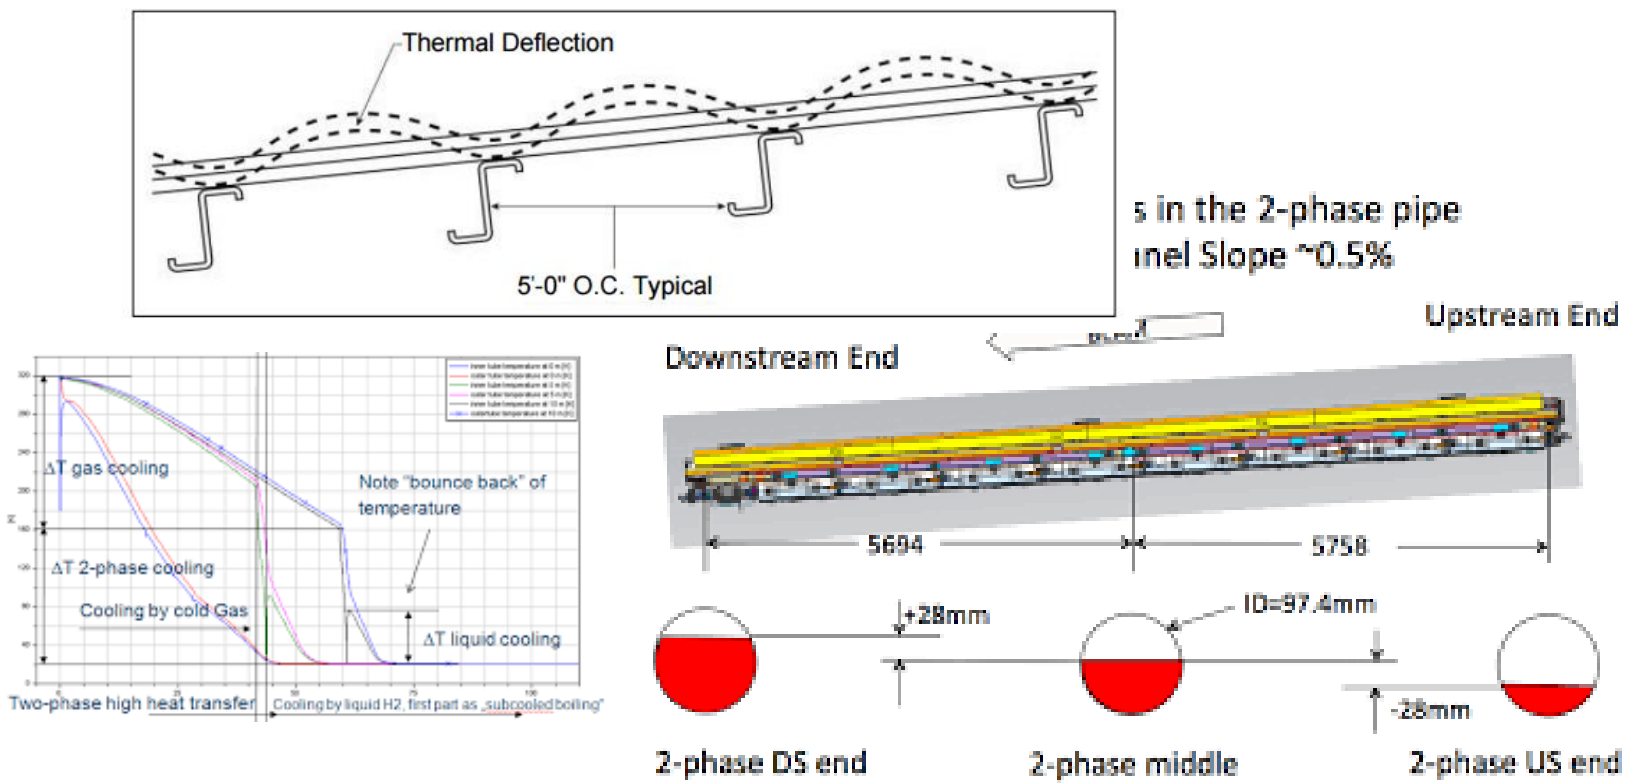
\includegraphics[width = \textwidth]{img/figure59.png}
    \caption{Thermal bowing.}
\end{figure}
\subsubsection{Laterial variation of temperature}
Thermal bowing occurs due to two processes:
\begin{enumerate}
    \item Restrained thermal expansion
    \item Temperature gradient across pipe
\end{enumerate}
Assuming no mean temperature increase:
\begin{equation}
    \Delta T = 0
\end{equation}
\begin{figure}[H]
    \centering
    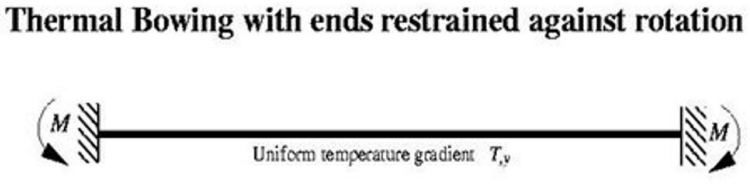
\includegraphics[width = 0.6\textwidth]{img/figure60.png}
    \caption{Fixed end beam subjected to a uniform thermal gradient.}
\end{figure}
Uniform moment over the length:
\begin{equation}
    M = EI \phi = EI\alpha T_{,y}
\end{equation}
\begin{figure}[H]
    \centering
    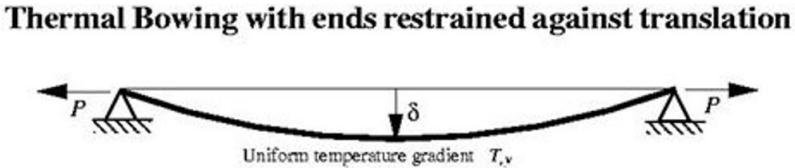
\includegraphics[width = 0.6\textwidth]{img/figure61.png}
    \caption{Laterally restrained beam subjected to a uniform thermal gradient.}
\end{figure}
A tensile force $P$ will be generated causing a tensile $P-\delta$ moment $Py$ over the length of the beam,
\begin{equation}
    \frac{\dif^2 y}{\dif x^2} = \phi + \frac{Py}{EI}
\end{equation}
or
\begin{equation}
    \frac{\dif^2 y}{\dif x^2} - k^2 y = \phi
\end{equation}
where,
\begin{equation}
    K = \sqrt{\frac{P}{EI}}
\end{equation}
The solution of this equation is,
\begin{equation}
    y\left(x\right) = -\frac{\phi}{k^2}\left(\frac{\cosh\left(kl\right) - 1}{\sinh\left(kl\right)}\sinh\left(kx\right)\cosh\left(kx\right)+1\right)
\end{equation}
\subsubsection{Derivation}
The derivation starts with the point that the displacement is:
\begin{equation}
    u = f\left(x\right) + yf_1\left(x\right) + zf_2\left(x\right)
\end{equation}
The longitudinal strain is
\begin{equation}
    \epsilon_{xx} = \frac{\partial u}{\partial x} = f'\left(x\right) + yf_1'\left(x\right) + zf_2'\left(x\right)
\end{equation}
The stress field is
\begin{equation}
    \sigma_{xx} = E \left(\epsilon_{xx} - \alpha T\right)
\end{equation}
The equilibrium constraints are
\begin{align}
    \int \sigma \dif A   & = 0 \\
    \int \sigma y \dif A & = 0 \\
    \int \sigma z \dif A & = 0
\end{align}
The geometrical constraint is
\begin{equation}
    \int y \dif A = \int z \dif A = 0
\end{equation}
Cross-pipe variation of temperature:
\begin{equation}
    \sigma_{xx} = -\alpha E\left(T - \bar{T}\right) + \frac{I_yM_{Tz}-I_{yx}M_{Ty}}{I_yI_z-I^2_{yz}}y + \frac{I_yM_{Tz}-I_{yx}M_{Ty}}{I_yI_z-I^2_{yz}}z
\end{equation}
where
\begin{align}
    I_z    & = \int y^2 \dif A        \\
    I_y    & = \int z^2 \dif A        \\
    I_{yz} & = \int yz \dif A         \\
    M_{Ty} & = \int \alpha ETz \dif A \\
    M_{Tz} & = \int \alpha ETy \dif A
\end{align}
For a pipe
\begin{equation}
    \sigma_{xx} = -\alpha E \left(T - \bar{T}\right) + \frac{M_{Tz}}{I_y}y
\end{equation}
For the lateral displacement
\begin{gather}
    \frac{\dif^2 v}{\dif x^2} = - \frac{M_{Tz}}{EI_z}\\
    \frac{\dif}{\dif x^2}\left(EI_z\frac{\dif^2 v}{\dif x^2}\right) + \frac{\dif^2 M_{Tz}}{\dif x^2} = F
\end{gather}
\begin{figure}[H]
    \centering
    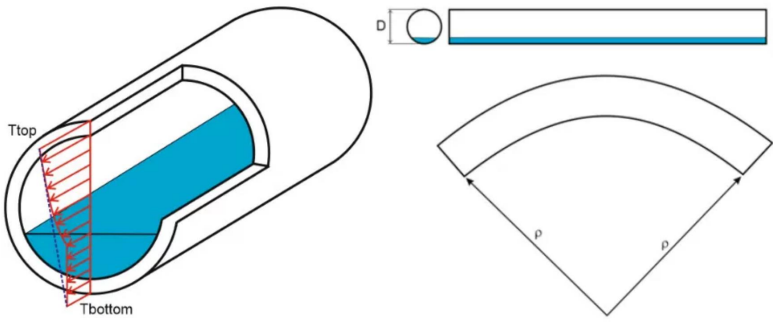
\includegraphics[width = 0.6\textwidth]{img/figure62.png}
    \caption{Cross-section of pipe.}
\end{figure}
\section{Phase change transition}
NG Rapid Phase Transitions (RPT). Rapid changes in phase due to temperature leads to enormous fluid impulse. This causes problems with the piping network. Rapid phase changes leads to a fluid impulse and often regarded as a water hammer. This phenomenon is well known in the context of steam (from the 19$^{\textrm{th}}$ century) - leading it to be called the steam hammer.

In a steam system, a water hammer most often occurs when some of the steam condenses into water in a horizontal section of the piping. The rest of the steam picks up the water, forming a ``slug'', and hurls this at high velocity into a pipe fitting, creating a loud hammering noise and greatly stressing the pipe. This condition is usually caused by a poor condensate drainage strategy: having more condensate in the pipe makes the slug easier to form. Vacuum caused by condensation from the thermal shock can also cause a steam hammer. Steam hammers can be avoided by using sloped pipes and installing steam traps. Where air-filled traps are used, these eventually become depleted of their trapped air over a long period through absorption into the water. This can be  cured by shutting off the supply, opening taps at the highest and lowest locations to drain the system (thereby restoring air to the lowest traps), and then closing the taps and re-opening the supply. 
\section{LNG transport}
The various stages need to be analysed. The first is the transport in the pipe. The second is the filling the space. The third is the environmental challenges - phase change water hammer. 
\subsubsection{Moss tanks}
Named after the company that designed them, the Norwegian company Moss Maritime, the spherical IMO type B LNG tanks are spherical in shape. Most Moss type vessels have four or five tanks. 

The outside of the tank has a thick layer of foam insulation that is either fitted in panels or in more modern designs, wound round tank. Over this insulation is a thin layer of ``tinfoil'' which allows the insulation to be kept dry with a nitrogen atmosphere. This atmosphere is constantly checked for any methane that would indicate a leak of the tank. Also the outside of tank is checked at three month intervals for any cold spots that would indicate breakdown in the insulation.

The tank is supported around its circumference by the equatorial ring which is supported by a large circular skirt which takes the weight of the tank down to the ships structure. This skirt allows the tank to expand and contract during cool-down and warm-up operations. During cool-down or warm-up, the tank can expand or contract about \SI{60}{\centi\meter}. Because of this expansion and contraction all piping into the tank comes in the top and is connected to the ships lines via flexible bellows. 

Inside ach tank there is a set of spray heads. These heads are mounted around the equatorial ring and are used to spray liquid LNG onto the tank walls to reduce the temperature. 

Tanks normally have a working pressure of up to \SI{22}{\kilo\pascal}, but this can be raised for an emergency discharge. If both main pumps fail then to remove cargo, the tank's safety valves are adjusted to lift at \SI{1}{bar}. Then the filling line which goes to the bottom of the tank is opened along with the filling lines of the other tanks on board. THe pressure is then raised in the tank with the defective pumps which pushes the cargo into the other tanks where it can be pumped out.
\subsubsection{TGZ Mark III}
Designed by Technigaz, these tanks are of the membrane type. The membrane consists of stainless steel with `waffles' to absorb the thermal contraction when the tank is cooled down. The primary barrier, made of corrugated stainless steel of about \SI{1.2}{\milli\meter} thickness is the one in direct contact with the cargo liquid (or vapour in the empty tank condition). This is followed by a primary insulation which in turn is covered by a secondary barrier made of a material called `triplex' which is basically a metal foil sandwiched between glasswool sheets and compressed together. This is again covered by a secondary insulation which in turn is supported by the ship's hull structure from the outside. 

From the inside of the tank outwards, the layers are:
\begin{enumerate}
    \item LNG
    \item Primary barrier of \SI{1.2}{\milli\meter} thick corrugated / waffled 304L stainless steel
    \item Primary insulation (also called the interbarrier space)
    \item Secondary barrier within the triplex membrane
    \item Secondary insulation (also called the insulation space)
    \item Ship's hull structure
\end{enumerate}
\begin{figure}[H]
    \centering
    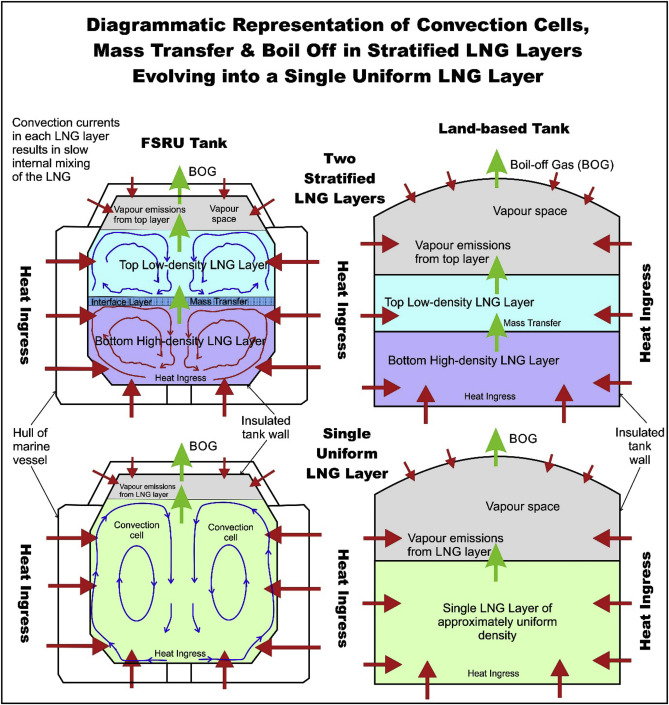
\includegraphics[width = 0.8\textwidth]{img/figure63.jpg}
    \caption{LNG rollover.}
\end{figure}
LNG ``rollover'' refers to the rapid release of LNG vapours from a storage tank caused by stratification. The potential for rollover arises when two separate layers of different densities (due to different LNG compositions) exist in a tank. In the top layer, liquid warms up due to heat leakage into the tank, rises up to the surface, where it evaporates. Thus light gases are preferentially evaporated and the liquid in the upper layer becomes denser. This phenomenon is called ``weathering''. In the bottom layer, the warmed liquid rises to the interface by free convection but does not evaporate due to the hydrostatic head exerted by the top layer. Thus the lower layer becomes warmer and less dense. As the density of two layers approach each other, the two layers mix rapidly, and the lower layer which has been superheated gives off large amount of vapour as it rises to the surface of the tank.
\subsubsection{Reduction of explosion risk}
Tanks are filled via a series of stages
\begin{enumerate}
    \item Flush tank with \ce{CO2} from the exhaust. This is because LNG and air mixture is flammable
    \item Fill with LNG at ambient temperature and pressure
    \item Vessel goes into port to ``gas-up'' and ``cool-down'', as one still cannot load directly into the tank: the \ce{CO2} will freeze and damage the pumps and the cold shock could damage the tank's pump column
    \item LNG is brought onto the vessel and taken along the spray line to the main vaporiser, which boils off the liquid into gas. This is then warmed up to roughly \SI{20}{\degree C} in the gas heaters and then blown into the tanks to displace the ``inert gas''. This continues until all the \ce{CO2} is removed from the tanks. Initially the IG (inert gas) is vented to atmosphere. Once the hydrocarbon content reaches 5\% (lower flammability range of methane) the inert gas is redirected to shore via a pipeline and manifold connection by the HD (high duty) compressors. This shore terminal then burns this vapour to avoid the dangers of having large amounts of hydrocarbons around which may explode
    \item Now the vessel is gassed up and warm. The tanks are still at ambient temperature and are full of methane
    \item The next stage is cool-down. LNG is sprayed into the tanks via spray heads, which vaporises and starts to cool the tank. The excess gas is again blown ashore to be re-liquefied or burned at a flare stack. Once the tanks reach about \SI{-140}{\degree C} the tanks are ready to load bulk
    \item Bulk loading starts and liquid LNG is pumped from the storage tanks ashore into the vessel tanks. Displaced gas is blown ashore by the HD compressors. Loading continues until typically 98.5\% full is reached (to allow for thermal expansion / contraction of cargo)
    \item The vessel can now proceed to the discharge port. During passage, various boil-off management strategies can be used. Boil-off gas can be burned in boilers to provide steam for propulsion, or it can be re-liquefied and returned to the cargo tanks, depending on the design of the vessel
\end{enumerate}
\subsubsection{Above ground full containment LNG tank design}
\begin{figure}[H]
    \centering
    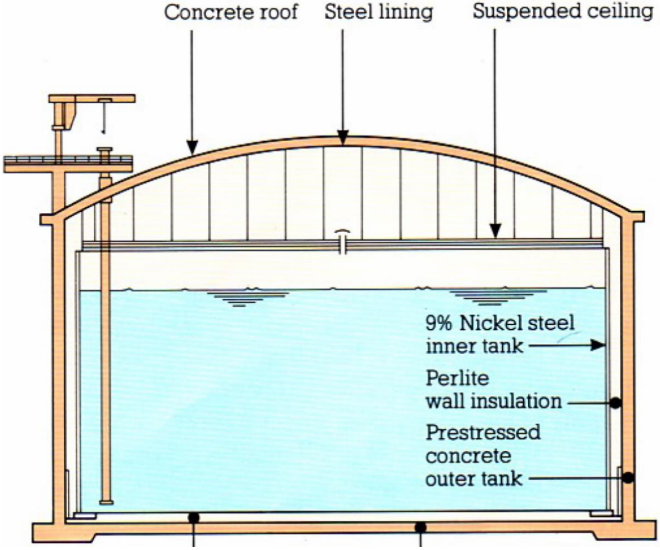
\includegraphics[width = 0.6\textwidth]{img/figure64.png}
    \caption{Above ground full containment LNG tank design.}
\end{figure}
\begin{itemize}
    \item Pre-stressed concrete outer walls constructed by slipforming, sheathed internally with a gas-tight layer of nickel-alloyed steel
    \item Inner tank in nickel-alloyed steel, separated from the outer walls by a layer of perlite - a variety of volcanic obsidian highly suitable for insulation
    \item Extra layer of steel and insulation at the transition between outer wall and tank bottom to protect it against strong local stresses should the inner tank begin to leak
    \item Heating cables under the tanks will ensure that ground remains above \SI{0}{\degree C} in order to prevent frost heaving
\end{itemize}
\subsubsection{Rollover}
Rollover is a phenomenon that can occur when LNG at different density / temperature is filled into a storage tank. LNG composition, density and temperature will change during boil-off gas. If not mixed, a high density liquid will settle below the lower density liquid. During heat leakage and evaporation, the density of the upper level of liquid can become higher than the lower level of liquid and a sudden rollover with mixing of the liquids may occur giving sudden evaporation and pressure build up, which can lead to tank rupture. In 1971, a rollover incident happened at the La Spezia LNG import terminal in Italy and damaged the tank roof. No ignition happened. Receiving terminals now have procedures to mix old and new LNG during filling. LNG tanks have rollover protection systems which include distributed temperature sensors and pump-around mixing systems.
\begin{figure}[H]
    \centering
    \includegraphics[width = 0.8\textwidth]{img/figure65.png}
    \caption{Mechanics of rollover in LNG tanks.}
\end{figure}
\begin{figure}[H]
    \centering
    \includegraphics[width = 0.8\textwidth]{img/figure66.png}
    \caption{Measurement of LNG density in tank.}
\end{figure}
\section{Sub 4K refrigeration system}
Cooling using a refrigeration system. Also can use paramagnetic materials. Helium is expensive so everything is recovered. Usually \ce{He} is delivered at \SI{4.5}{\kelvin} \SI{3}{bar}. \SI{2}{\kelvin} helium is produced by a cryogenic device. Issue to do with pressure for a helium transport. 
\subsubsection{Transfer lines}
Cryogenic transfer lines are modular. They usually consist of multichannel components.
\begin{enumerate}
    \item Thermal shield
    \item External envelope
    \item Vacuum barrier
    \item Sliding support
    \item Fixed supports
\end{enumerate}
Both process and external envelope contain internal bellows to account for the shrinkage of pipes.
\begin{figure}[H]
    \centering
    \includegraphics[width = 0.8\textwidth]{img/figure67.png}
    \caption{Cryogenic transfer line cross-section and sliding support mechanism.}
\end{figure}
\begin{figure}[H]
    \centering
    \includegraphics[width = 0.8\textwidth]{img/figure68.png}
    \caption{Cryogenic transfer line components.}
\end{figure}
\begin{table}[H]
    \centering
    \includegraphics[width = \textwidth]{img/figure69.png}
    \caption{Sizes and operating conditions of the process lines, thermal shield and vacuum jacket.}
\end{table}
\subsubsection{SS304}
Type 304 stainless steel is a T 300 Series Stainless Steel austenitic. It has a minimum of 18\% chromium and 8\% nickel, combined with a maximum of 0.08\% carbon. It is defined as a Chromium-Nickel austenitic alloy. Grade 304 is the standard ``18/8'' stainless that you will probably see in your pans and cookery tools. These are some of its characteristics:
\begin{itemize}
    \item Forming and welding properties
    \item Corrosion / oxidation resistance thanks to chromium content
    \item Deep drawing quality
    \item Excellent toughness, even down to cryogenic temperatures, which are defined as very low temperatures
    \item Low temperature properties responding well to hardening by cold working
    \item Ease of cleaning, ease of fabrication, beauty of appearance
    \item Grade 304L is the low carbon version of 304. It does not require post-weld annealing and so is extensively using heavy gauge components (over about \SI{6}{\milli\meter})
    \item Grade 304H with its higher carbon content finds application at elevated temperatures
\end{itemize} 
\part{Extreme Corrosion}
\chapter{Corrosion Classification}
\section{Extreme environments}
We study the influence of slow and fast chemistry on structures. Mediated through chemistry that occurs on the surface of materials. This is generally through electrochemical processes that are generally associated with corrosion. Corrosion covers a vast area of material science so we must first go through some of the key electrochemical processes which we cover in this lecture. We are generally interested in the long term view.
\section{Corrosion}
Corrosion is defined as the conversion of metal to a more chemically stable form by chemical and / or electrochemical reaction with their environment. Metals are susceptible because they are good conductors. Corrosion degrades the useful properties of material and structures including strength.
\subsection{Corrosion is similar to a battery}
\begin{figure}[H]
    \centering
    \includegraphics[width = 0.8 \textwidth]{img/figure70.png}
    \caption{Corrosion mechanism compared to battery.}
\end{figure}
This requires an exchange and so only occurs when there are differences. This is classified as either:
\begin{enumerate}
    \item Two different metals in the same liquid
    \item Two different liquids with the same metal
\end{enumerate}
To understand how to stop corrosion, we will have two choices - either coat materials or understand why reaction occurs. First step is to understand the basics of electrochemistry - chemistry is an exchange of electrons. If something is oxidised then something else must be reduced. Reactivity depends what is in the aqueous mixture in contact with the metal.
\subsection{Electrode potentials}
\begin{figure}[H]
    \centering
    \includegraphics[width = 0.5 \textwidth]{img/figure71.png}
    \caption{Copper reduction and iron oxidation setup in galvanic cell.}
    \label{copperRedIronOx}
\end{figure}
If the iron and copper electrodes are connected electrically, reduction will occur for copper at the expense of the oxidation of iron. \ce{Cu^2+} ions will deposit (electrodeposit) as metallic copper on the copper electrode, while iron dissolves (corrodes) on the other side of the cell and goes into solution.
\begin{align}
    \ce{Fe -> Fe^2+ + 2e^-} \qquad       & \textrm{(oxidation)}        \\
    \ce{Cu^2+ + 2e^- -> Cu} \qquad       & \textrm{(reduction)}        \\
    \ce{Cu^2+ + Fe -> Cu + Fe^2+} \qquad & \textrm{(overall reaction)}
\end{align}
\subsection{Salt bridge}
A salt bridge is used to connect the oxidation and reduction half-cells of a galvanic cell (voltaic cell), a type of electrochemical cell. It maintains electrical neutrality within the internal circuit, preventing the cell from reaction. Salt bridges usually come in two types:
\begin{enumerate}
    \item Glass tube - U-shaped glass tube filled with a relatively inert electrolyte; usually potassium chloride or sodium chloride is used (agar is often used as a gelification agent), although Figure \ref{copperRedIronOx} here illustrates the use of a potassium nitrate solution. The conductivity of the glass tube bridge depends mostly on the concentration of the electrolyte solution. An increase in concentration below saturation increases conductivity. Beyond-saturation electrolyte content and narrow tube diameter may both lower conductivity
    \item Filter paper - the other type of salt bridge consists of filter paper, also soaked with a relatively inert electrolyte, usually potassium chloride or sodium chloride because they are chemically inert. No gelification agent is required as the filter paper provides a solid medium for conduction. Conductivity of this kind of salt bridge depends on a number of factors: the concentration of the electrolyte solution, the texture of the filter paper and the absorbing ability of the filter paper. Generally smoother texture and higher absorbency equates to higher conductivity
\end{enumerate}
\subsection{Electrochemical considerations}
\subsubsection{Oxidation reaction}
Metal atoms characteristically lose or give up electrons in what is called an oxidation reaction.
\begin{equation}
    \ce{M -> M^n+ + ne^-}
\end{equation}
where \ce{n} is valence (number of valent electrons). the site at which oxidation takes place is called the anode. Oxidation is sometimes called an anodic reaction. Example:
\begin{gather}
    \ce{Fe(s) -> Fe^2+(aq) + 2e^-}\\
    \ce{Al(s) -> Al^3+(aq) + 3e^-}
\end{gather}
\subsubsection{Reduction reaction}
The electrons from each oxidised metal atom must be transferred to and become a part of another chemical species in what is termed a reduction reaction. In acid solutions, which have a high concentration of hydrogen ions:
\begin{equation}
    \ce{2H^+ + 2e^- -> H2(g)}
\end{equation}
pH = $- \log_{10}\left[\ce{H^+}\right]$, where more \ce{H^+} results in pH $<$ 7. For an acid solution having dissolved oxygen:
\begin{equation}
    \ce{O2 + 4H^+ + 4e^- -> 2H2O}
\end{equation}
For a neutral or basic aqueous solution in which oxygen is dissolved:
\begin{equation}
    \ce{O2 + 2H2O + 4e^- -> 4OH^-}
\end{equation}
Any metal ions present in the solution may be reduced:
\begin{gather}
    \ce{M^n+ + ne^- -> M}
\end{gather}
The location at which reduction occurs is called the cathode. It is possible for two or more of the reduction reactions to occur simultaneously.
\subsection{Galvanic couple}
Two metals electrically connected in a liquid electrolyte wherein one metal becomes an anode and corrodes while the other acts as a cathode.

The question is which one corrodes. An electric potential or voltage will exist between the two cell halves, and its magnitude can be determined if a voltmeter is connected in the external circuit. Various electrode pairs have different voltages; the magnitude of such a voltage may be thought of as representing the driving force for the electrochemical oxidation-reduction reaction.
\begin{align}
    \ce{Cu^2+ + Fe -> Cu + Fe^2+} \quad & \left(\SI{0.780}{\volt}\right) \\
    \ce{Fe^2+ + Zn -> Fe + Zn^2+} \quad & \left(\SI{0.323}{\volt}\right)
\end{align}
Standard half cell: a half-cell of a metal electrode immersed in a \ce{1M} solution of ions and at \SI{25}{\degree C}. To understand reaction, we have to look at one half of the electrochemical cell or half-battery, specifically when one half of the battery is a standard form.
\section{Standard hydrogen reference probe}
It consists of an inert platinum electrode in a \ce{1M} solution of \ce{H^+} ions, saturated with hydrogen gas that is bubble through the solution at a pressure of \SI{1}{atm} and a temperature of \SI{25}{\degree C}.

\textbf{Standard electromotive force (emf) series.} It is generated by coupling to the standard hydrogen electrode, standard half-cells for various metals and ranking them according to the measured voltage. This tells us the potential for reaction but not the rate.
\begin{figure}[H]
    \centering
    \includegraphics[width = 0.5 \textwidth]{img/figure72.png}
    \caption{Standard hydrogen reference probe.}
\end{figure}
\subsection{Standard emf series}
\begin{table}[H]
    \centering
    \begin{tabular}{@{}lll@{}}
        \toprule
                            & \textbf{Electrode reaction}    & \textbf{Standard electrode}           \\
                            & \textbf{(reduction)}           & \textbf{potential} $V^0$ (\si{\volt}) \\
        \midrule
        Reduction (cathode) & \ce{Au^3+ + 3e^- -> Au}        & +1.420                                \\
                            & \ce{O_s + 4H^+ + 4e^- -> 2H2O} & +1.229                                \\
                            & \ce{Pt^2+ + 2e^- -> Pt}        & +1.200                                \\
                            & \ce{Fe^3+ + e^- -> Fe^2+}      & +0.771                                \\
                            & \ce{Cu^2+ + 2e^- -> Cu}        & +0.340                                \\
                            & \ce{Fe^2+ + 2e^- -> Fe}        & -0.440                                \\
                            & \ce{Zn^2+ + 2e^- -> Zn}        & -0.763                                \\
                            & \ce{Na^+ + e^- -> Na}          & -2.714                                \\
        Oxidation (anode)   & \ce{K^+ + e^- -> K}            & -2.924                                \\
        \bottomrule
    \end{tabular}
    \caption{Table to show standard emf series. Increasingly inert to increasingly reactive from top to bottom. E.g. With \ce{Cu} and \ce{Fe}, \ce{Fe} corrodes. With \ce{Fe} and \ce{Zn}, \ce{Zn} corrodes.}
\end{table}
\section{Classification of corrosion types}
\begin{figure}[H]
    \centering
    \includegraphics[width = \textwidth]{img/figure73.png}
    \caption{Classification of corrosion types.}
\end{figure}
\subsection{Group 1: corrosion you can see}
\begin{enumerate}
    \item Uniform corrosion characterised by even, regular loss of metal from corroding surface
    \item Localised corrosion during which most of metal loss occurs at discrete areas. This includes crevice corrosion, pitting
    \item Galvanic corrosion occasioned by electrical contact between dissimilar conductors in an electrolyte
\end{enumerate}
\subsection{Group 2: multiple mechanisms}
\begin{enumerate}
    \item Erosion - corrosion. Usually high speed flow with particles, cavitation with bubbles near walls, friction and fretting
    \item Intergranular corrosion at grain boundaries in the metal structure (grains acts a bit like local galvanic couples). Common occurrence which is called weld decay
    \item Dealloying corrosion (selecting leaching) due to selective dissolution of one component of an alloy (e.g. zinc from brass alloy with \ce{O2} and moisture, iron from cast iron)
\end{enumerate}
\subsection{Group 3: microscope corrosion viewed by microscope}
\begin{enumerate}
    \item Corrosion fatigue. Small cracks are enlarged by corrosion and fatigue which then affects the crack growth. Tensile stresses propagate the crack. Corrosion further deteriorate crack
    \item High-temperature corrosion (scaling, internal attack, oxygen corrosion of nickel)
    \item Microbial effects caused by certain bacteria when their metabolism created corrosive elements and deposits. Sulfate-reducing bacteria
\end{enumerate}
\begin{figure}[H]
    \centering
    \includegraphics[width = \textwidth]{img/figure74.png}
    \caption{Frequency of different corrosion types.}
\end{figure}
\section{Corrosion mechanisms in-depth}
\subsection{Pitting corrosion}
Creation of small holes in materials which can perforate thin sheets. This is an example of where there is one metal but two types of electrolyte in the vicinity of the metal. This is because the reaction within the hole or pit is not the same as the reaction outside. Pitting results when a small hole or cavity forms in the metal, usually as a result of de-passivation of a small area. This area becomes anodic, while part of the remaining metal becomes cathodic, producing a localised galvanic reaction. The deterioration of this small area penetrates the metal and can lead to failure. This form of corrosion is often difficult to detect due to the fact that it is usually relatively small and may be covered and hidden by corrosion-produced compounds.

Certain conditions, such as low concentrations of oxygen or high concentrations of chloride which complete as anions, can interfere with a given alloy's ability to re-form a passivating film. Corrosion at these points will be greatly amplified, and can cause corrosion pits of several types, depending upon conditions. While the corrosion pits only nucleate under fairly extreme circumstances, they can continue to grow even when conditions return to normal, since the interior of a pit is naturally deprived of oxygen and locally the pH decreases to very low values and the corrosion rate increases due to an autocatalytic process. In extreme cases, the sharp tips of extremely long and narrow corrosion pits can cause stress concentration to the point that otherwise tough alloys can shatter; a thin firm pierced by an invisibly small hole can hide a thumb sized pit from view. These problems care especially dangerous because they are difficult to detect before a part or structure fails. Pitting remains among the most common and damaging forms of corrosion in passivated alloys, but it can be prevented by control of the alloy's environment.

Pitting is autocatalytic in nature. Once a pit starts to grow, the conditions developed are such that further pit growth is promoted. The anodic and cathodic electrochemical reactions that comprise corrosion separate spatially during pitting. The local pit environment becomes depleted in cathodic reactant (e.g. oxygen), which shifts most of the cathodic reaction to the boldly exposed surface where this reactant is more plentiful. The pit environment becomes enriched in metal cations and an anionic species such as chloride, which electromigrates into the put to maintain charge neutrality by balancing the charge associated with the cation concentration. The pH in the pit is lower owing to cation hydrolysis.
\begin{enumerate}
    \item The formation of anodic sits by disruption of the protective passive film on the metal surface.
          \begin{equation}
              \ce{M -> M^n+ + ne^-}
          \end{equation}
          This is balanced by the cathodic reaction of oxygen on the adjacent surface
          \begin{equation}
              \ce{O2 + 2H2O + 4e^- -> 4OH^-}
          \end{equation}
    \item Due to the continuing metal dissolution, an excess of positive ions (\ce{M^n+}) is accumulated in the anodic area. The process is self-stimulating and self-propagating. To maintain charge neutrality negative ions (anions), like chloride, migrate from electrolyte (for example, seawater of a 5\% \ce{NaCl} solution).
          \begin{equation}
              \ce{M^+Cl^- + H2O -> MOH + H^+Cl^-}
          \end{equation}
          \ce{OH^-} ions also migrate to neutralise the positive charges. This process is called hydrolysis
    \item The presence of (\ce{H^+}) ions and chloride content, prevents repassivation. The above the process generates free acid and the pH value at the bottom of pit is substantially lowered (1.5-1.0)
    \item The increase in the rate of dissolution at the anode increases the rate of migration of the chloride ions and the reaction becomes time dependent and continues, resulting in the formation of more and more \ce{M^+Cl^-}, generation of more and more \ce{H^+Cl^-} by hydrolysis
    \item The process continues until the metal is perforated. The process is autocatalytic and it increases with time resulting in more and more dissolution
    \item Finally, the metal is perforated and the reaction is terminated
\end{enumerate}
\begin{figure}[H]
    \centering
    \includegraphics[width = \textwidth]{img/figure75.png}
    \caption{Pitting corrosion.}
\end{figure}
\subsection{Crevice corrosion}
Crevice corrosion is a localised form of corrosion occurring in confined spaces (crevices), to which the access of the working fluid from the environment is limited. Formation of a differential aeration cells leads to corrosion inside the crevices. Examples of crevices are gaps and contact areas between parts, under gaskets or seals, inside cracks and seams, spaces filled with deposits and under sludge pile.

Crevice corrosion is influenced by the crevice type (metal-metal, metal-non-metal), crevice geometry (size, surface finish) and metallurgical and environmental factors. The susceptibility to crevice corrosion can be evaluated with ASTM standard procedures. A critical crevice corrosion temperature is commonly used to rank a material's resistance to crevice corrosion.
\subsubsection{Mechanism}
\begin{figure}[H]
    \centering
    \includegraphics[width = 0.8\textwidth]{img/figure76.png}
    \caption{Mechanism of crevice corrosion.}
\end{figure}
Crevice corrosion is initiated by a difference between some chemical constituents, usually oxygen, which sets up an electrochemical concentration cell. Outside of the crevice (the cathode), the oxygen content and pH are higher - but chlorides are lower.

Chlorides concentrate inside the crevice (the anode) worsening the situation. Ferrous ions forms ferric chloride and attack the stainless steel rapidly. The pH and oxygen content are lower inside the crevice (can be as low as 2). Once the crevice has formed the propagation mechanism continues.
\begin{figure}[H]
    \centering
    \includegraphics[width = 0.8\textwidth]{img/figure77.png}
    \caption{Chronology of crevice corrosion.}
\end{figure}

%\newpage
%\bibliographystyle{unsrtnat}
%\bibliography{Refs.bib}
%\appendix
\chapter{Plots}
\begin{figure}[H]
    \centering
    \includegraphics[width = 0.8\textwidth]{img/Roll Type.pdf}
    \caption{RMSE results for Type-1 and Type-2 Configurations for Roll Output}
    \label{fig:roll_type}
\end{figure}
\begin{figure}[H]
    \centering
    \includegraphics[width = 0.8\textwidth]{img/Pitch Type.pdf}
    \caption{RMSE results for Type-1 and Type-2 Configurations for Pitch Output}
    \label{fig:pitch_type}
\end{figure}
\begin{figure}[H]
    \centering
    \includegraphics[width = 0.6\textwidth]{img/Yaw Type2.pdf}
    \caption{RMSE results for Type-1 and Type-2 Configurations for Yaw Output}
    \label{fig:yaw_type}
\end{figure}
\begin{figure}[H]
    \centering
    \includegraphics[width = 0.6\textwidth]{img/Thrust Type.pdf}
    \caption{RMSE results for Type-1 and Type-2 Configurations for Thrust Output}
    \label{fig:thrust_type}
\end{figure}
\begin{figure}[H]
    \centering
    \begin{minipage}[b]{0.45\textwidth}
        \includegraphics[height=5cm,keepaspectratio]{img/scenario1_pid_paths.eps}
        \caption{Scenario 1 Path taken using PID Drone Control}
        \label{fig:Paths1_pid}
    \end{minipage}
    \hfill
    \begin{minipage}[b]{0.45\textwidth}
        \includegraphics[height=5cm,keepaspectratio]{img/scenario1_fis_paths.eps}
        \caption{Scenario 1 Path taken using ANFIS Drone Control}
        \label{fig:Paths1_fis}
    \end{minipage}
\end{figure}
\begin{figure}[H]
    \centering
    \begin{minipage}[b]{0.45\textwidth}
        \includegraphics[height=5cm,keepaspectratio]{img/scenario2_pid_paths.eps}
        \caption{Scenario 2 Path taken using PID Drone Control}
        \label{fig:Paths2_pid}
    \end{minipage}
    \hfill
    \begin{minipage}[b]{0.45\textwidth}
        \includegraphics[height=5cm,keepaspectratio]{img/scenario2_fis_paths.eps}
        \caption{Scenario 2 Path taken using ANFIS Drone Control}
        \label{fig:Paths2_fis}
    \end{minipage}
\end{figure}
\begin{figure}[H]
    \centering
    \begin{minipage}[b]{0.45\textwidth}
        \includegraphics[height=5cm,keepaspectratio]{img/scenario3_pid_paths.eps}
        \caption{Scenario 3 Path taken using PID Drone Control}
        \label{fig:Paths3_pid}
    \end{minipage}
    \hfill
    \begin{minipage}[b]{0.45\textwidth}
        \includegraphics[height=5cm,keepaspectratio]{img/scenario3_fis_paths.eps}
        \caption{Scenario 3 Path taken using ANFIS Drone Control}
        \label{fig:Paths3_fis}
    \end{minipage}
\end{figure}
\begin{figure}[H]
    \centering
    \begin{minipage}[b]{0.45\textwidth}
        \includegraphics[height=5cm,keepaspectratio]{img/scenario4_pid_paths.eps}
        \caption{Scenario 4 Path taken using PID Drone Control}
        \label{fig:Paths4_pid}
    \end{minipage}
    \hfill
    \begin{minipage}[b]{0.45\textwidth}
        \includegraphics[height=5cm,keepaspectratio]{img/scenario4_fis_paths.eps}
        \caption{Scenario 4 Path taken using ANFIS Drone Control}
        \label{fig:Paths4_fis}
    \end{minipage}
\end{figure}
\begin{figure}[H]
    \centering
    \begin{minipage}[b]{0.45\textwidth}
        \includegraphics[height=5cm,keepaspectratio]{img/scenario5_pid_paths.eps}
        \caption{Scenario 5 Path taken using PID Drone Control}
        \label{fig:Paths5_pid}
    \end{minipage}
    \hfill
    \begin{minipage}[b]{0.45\textwidth}
        \includegraphics[height=5cm,keepaspectratio]{img/scenario5_fis_paths.eps}
        \caption{Scenario 5 Path taken using ANFIS Drone Control}
        \label{fig:Paths5_fis}
    \end{minipage}
\end{figure}

\end{document}